
%% bare_jrnl_compsoc.tex
%% V1.4b
%% 2015/08/26
%% by Michael Shell
%% See:
%% http://www.michaelshell.org/
%% for current contact information.
%%
%% This is a skeleton file demonstrating the use of IEEEtran.cls
%% (requires IEEEtran.cls version 1.8b or later) with an IEEE
%% Computer Society journal paper.
%%
%% Support sites:
%% http://www.michaelshell.org/tex/ieeetran/
%% http://www.ctan.org/pkg/ieeetran
%% and
%% http://www.ieee.org/

%%*************************************************************************
%% Legal Notice:
%% This code is offered as-is without any warranty either expressed or
%% implied; without even the implied warranty of MERCHANTABILITY or
%% FITNESS FOR A PARTICULAR PURPOSE! 
%% User assumes all risk.
%% In no event shall the IEEE or any contributor to this code be liable for
%% any damages or losses, including, but not limited to, incidental,
%% consequential, or any other damages, resulting from the use or misuse
%% of any information contained here.
%%
%% All comments are the opinions of their respective authors and are not
%% necessarily endorsed by the IEEE.
%%
%% This work is distributed under the LaTeX Project Public License (LPPL)
%% ( http://www.latex-project.org/ ) version 1.3, and may be freely used,
%% distributed and modified. A copy of the LPPL, version 1.3, is included
%% in the base LaTeX documentation of all distributions of LaTeX released
%% 2003/12/01 or later.
%% Retain all contribution notices and credits.
%% ** Modified files should be clearly indicated as such, including  **
%% ** renaming them and changing author support contact information. **
%%*************************************************************************


% *** Authors should verify (and, if needed, correct) their LaTeX system  ***
% *** with the testflow diagnostic prior to trusting their LaTeX platform ***
% *** with production work. The IEEE's font choices and paper sizes can   ***
% *** trigger bugs that do not appear when using other class files.       ***                          ***
% The testflow support page is at:
% http://www.michaelshell.org/tex/testflow/


\documentclass[10pt,journal,compsoc]{IEEEtran}
% \documentclass[10pt,compsoc,cspaper]{IEEEtran}
% \documentclass[10pt,peerreviewca,compsoc]{IEEEtran}
%.cls has not been installed into the LaTeX system files,
% manually specify the path to it like:
% \documentclass[10pt,journal,compsoc]{../sty/IEEEtran}





% Some very useful LaTeX packages include:
% (uncomment the ones you want to load)


% *** MISC UTILITY PACKAGES ***
%
%\usepackage{ifpdf}
% Heiko Oberdiek's ifpdf.sty is very useful if you need conditional
% compilation based on whether the output is pdf or dvi.
% usage:
% \ifpdf
%   % pdf code
% \else
%   % dvi code
% \fi
% The latest version of ifpdf.sty can be obtained from:
% http://www.ctan.org/pkg/ifpdf
% Also, note that IEEEtran.cls V1.7 and later provides a builtin
% \ifCLASSINFOpdf conditional that works the same way.
% When switching from latex to pdflatex and vice-versa, the compiler may
% have to be run twice to clear warning/error messages.






% *** CITATION PACKAGES ***
%
\ifCLASSOPTIONcompsoc
  % IEEE Computer Society needs nocompress option
  % requires cite.sty v4.0 or later (November 2003)
  \usepackage[nocompress]{cite}
\else
  % normal IEEE
  \usepackage{cite}
\fi
% cite.sty was written by Donald Arseneau
% V1.6 and later of IEEEtran pre-defines the format of the cite.sty package
% \cite{} output to follow that of the IEEE. Loading the cite package will
% result in citation numbers being automatically sorted and properly
% "compressed/ranged". e.g., [1], [9], [2], [7], [5], [6] without using
% cite.sty will become [1], [2], [5]--[7], [9] using cite.sty. cite.sty's
% \cite will automatically add leading space, if needed. Use cite.sty's
% noadjust option (cite.sty V3.8 and later) if you want to turn this off
% such as if a citation ever needs to be enclosed in parenthesis.
% cite.sty is already installed on most LaTeX systems. Be sure and use
% version 5.0 (2009-03-20) and later if using hyperref.sty.
% The latest version can be obtained at:
% http://www.ctan.org/pkg/cite
% The documentation is contained in the cite.sty file itself.
%
% Note that some packages require special options to format as the Computer
% Society requires. In particular, Computer Society  papers do not use
% compressed citation ranges as is done in typical IEEE papers
% (e.g., [1]-[4]). Instead, they list every citation separately in order
% (e.g., [1], [2], [3], [4]). To get the latter we need to load the cite
% package with the nocompress option which is supported by cite.sty v4.0
% and later. Note also the use of a CLASSOPTION conditional provided by
% IEEEtran.cls V1.7 and later.





% *** GRAPHICS RELATED PACKAGES ***
%
\ifCLASSINFOpdf
   \usepackage[pdftex]{graphicx}
%   declare the path(s) where your graphic files are
   \graphicspath{{../pdf/}{../jpeg/}}
%   and their extensions so you won't have to specify these with
%   every instance of \includegraphics
   \DeclareGraphicsExtensions{.pdf,.jpeg,.png}
\else
  % or other class option (dvipsone, dvipdf, if not using dvips). graphicx
  % will default to the driver specified in the system graphics.cfg if no
  % driver is specified.
   \usepackage[dvips]{graphicx}
%   declare the path(s) where your graphic files are
   \graphicspath{{../eps/}}
%   and their extensions so you won't have to specify these with
%   every instance of \includegraphics
   \DeclareGraphicsExtensions{.eps}
\fi
% graphicx was written by David Carlisle and Sebastian Rahtz. It is
% required if you want graphics, photos, etc. graphicx.sty is already
% installed on most LaTeX systems. The latest version and documentation
% can be obtained at: 
% http://www.ctan.org/pkg/graphicx
% Another good source of documentation is "Using Imported Graphics in
% LaTeX2e" by Keith Reckdahl which can be found at:
% http://www.ctan.org/pkg/epslatex
%
% latex, and pdflatex in dvi mode, support graphics in encapsulated
% postscript (.eps) format. pdflatex in pdf mode supports graphics
% in .pdf, .jpeg, .png and .mps (metapost) formats. Users should ensure
% that all non-photo figures use a vector format (.eps, .pdf, .mps) and
% not a bitmapped formats (.jpeg, .png). The IEEE frowns on bitmapped formats
% which can result in "jaggedy"/blurry rendering of lines and letters as
% well as large increases in file sizes.
%
% You can find documentation about the pdfTeX application at:
% http://www.tug.org/applications/pdftex






% *** MATH PACKAGES ***
%
\usepackage{amsmath}
% A popular package from the American Mathematical Society that provides
% many useful and powerful commands for dealing with mathematics.
%
% Note that the amsmath package sets \interdisplaylinepenalty to 10000
% thus preventing page breaks from occurring within multiline equations. Use:
%\interdisplaylinepenalty=2500
% after loading amsmath to restore such page breaks as IEEEtran.cls normally
% does. amsmath.sty is already installed on most LaTeX systems. The latest
% version and documentation can be obtained at:
% http://www.ctan.org/pkg/amsmath





% *** SPECIALIZED LIST PACKAGES ***
%
%\usepackage{algorithmic}
% algorithmic.sty was written by Peter Williams and Rogerio Brito.
% This package provides an algorithmic environment fo describing algorithms.
% You can use the algorithmic environment in-text or within a figure
% environment to provide for a floating algorithm. Do NOT use the algorithm
% floating environment provided by algorithm.sty (by the same authors) or
% algorithm2e.sty (by Christophe Fiorio) as the IEEE does not use dedicated
% algorithm float types and packages that provide these will not provide
% correct IEEE style captions. The latest version and documentation of
% algorithmic.sty can be obtained at:
% http://www.ctan.org/pkg/algorithms
% Also of interest may be the (relatively newer and more customizable)
% algorithmicx.sty package by Szasz Janos:
% http://www.ctan.org/pkg/algorithmicx




% *** ALIGNMENT PACKAGES ***
%
%\usepackage{array}
% Frank Mittelbach's and David Carlisle's array.sty patches and improves
% the standard LaTeX2e array and tabular environments to provide better
% appearance and additional user controls. As the default LaTeX2e table
% generation code is lacking to the point of almost being broken with
% respect to the quality of the end results, all users are strongly
% advised to use an enhanced (at the very least that provided by array.sty)
% set of table tools. array.sty is already installed on most systems. The
% latest version and documentation can be obtained at:
% http://www.ctan.org/pkg/array


% IEEEtran contains the IEEEeqnarray family of commands that can be used to
% generate multiline equations as well as matrices, tables, etc., of high
% quality.




% *** SUBFIGURE PACKAGES ***
%\ifCLASSOPTIONcompsoc
%  \usepackage[caption=false,font=footnotesize,labelfont=sf,textfont=sf]{subfig}
%\else
%  \usepackage[caption=false,font=footnotesize]{subfig}
%\fi
% subfig.sty, written by Steven Douglas Cochran, is the modern replacement
% for subfigure.sty, the latter of which is no longer maintained and is
% incompatible with some LaTeX packages including fixltx2e. However,
% subfig.sty requires and automatically loads Axel Sommerfeldt's caption.sty
% which will override IEEEtran.cls' handling of captions and this will result
% in non-IEEE style figure/table captions. To prevent this problem, be sure
% and invoke subfig.sty's "caption=false" package option (available since
% subfig.sty version 1.3, 2005/06/28) as this is will preserve IEEEtran.cls
% handling of captions.
% Note that the Computer Society format requires a sans serif font rather
% than the serif font used in traditional IEEE formatting and thus the need
% to invoke different subfig.sty package options depending on whether
% compsoc mode has been enabled.
%
% The latest version and documentation of subfig.sty can be obtained at:
% http://www.ctan.org/pkg/subfig




% *** FLOAT PACKAGES ***
%
%\usepackage{fixltx2e}
% fixltx2e, the successor to the earlier fix2col.sty, was written by
% Frank Mittelbach and David Carlisle. This package corrects a few problems
% in the LaTeX2e kernel, the most notable of which is that in current
% LaTeX2e releases, the ordering of single and double column floats is not
% guaranteed to be preserved. Thus, an unpatched LaTeX2e can allow a
% single column figure to be placed prior to an earlier double column
% figure.
% Be aware that LaTeX2e kernels dated 2015 and later have fixltx2e.sty's
% corrections already built into the system in which case a warning will
% be issued if an attempt is made to load fixltx2e.sty as it is no longer
% needed.
% The latest version and documentation can be found at:
% http://www.ctan.org/pkg/fixltx2e


%\usepackage{stfloats}
% stfloats.sty was written by Sigitas Tolusis. This package gives LaTeX2e
% the ability to do double column floats at the bottom of the page as well
% as the top. (e.g., "\begin{figure*}[!b]" is not normally possible in
% LaTeX2e). It also provides a command:
%\fnbelowfloat
% to enable the placement of footnotes below bottom floats (the standard
% LaTeX2e kernel puts them above bottom floats). This is an invasive package
% which rewrites many portions of the LaTeX2e float routines. It may not work
% with other packages that modify the LaTeX2e float routines. The latest
% version and documentation can be obtained at:
% http://www.ctan.org/pkg/stfloats
% Do not use the stfloats baselinefloat ability as the IEEE does not allow
% \baselineskip to stretch. Authors submitting work to the IEEE should note
% that the IEEE rarely uses double column equations and that authors should try
% to avoid such use. Do not be tempted to use the cuted.sty or midfloat.sty
% packages (also by Sigitas Tolusis) as the IEEE does not format its papers in
% such ways.
% Do not attempt to use stfloats with fixltx2e as they are incompatible.
% Instead, use Morten Hogholm'a dblfloatfix which combines the features
% of both fixltx2e and stfloats:
%
% \usepackage{dblfloatfix}
% The latest version can be found at:
% http://www.ctan.org/pkg/dblfloatfix




%\ifCLASSOPTIONcaptionsoff
%  \usepackage[nomarkers]{endfloat}
% \let\MYoriglatexcaption\caption
% \renewcommand{\caption}[2][\relax]{\MYoriglatexcaption[#2]{#2}}
%\fi
% endfloat.sty was written by James Darrell McCauley, Jeff Goldberg and 
% Axel Sommerfeldt. This package may be useful when used in conjunction with 
% IEEEtran.cls'  captionsoff option. Some IEEE journals/societies require that
% submissions have lists of figures/tables at the end of the paper and that
% figures/tables without any captions are placed on a page by themselves at
% the end of the document. If needed, the draftcls IEEEtran class option or
% \CLASSINPUTbaselinestretch interface can be used to increase the line
% spacing as well. Be sure and use the nomarkers option of endfloat to
% prevent endfloat from "marking" where the figures would have been placed
% in the text. The two hack lines of code above are a slight modification of
% that suggested by in the endfloat docs (section 8.4.1) to ensure that
% the full captions always appear in the list of figures/tables - even if
% the user used the short optional argument of \caption[]{}.
% IEEE papers do not typically make use of \caption[]'s optional argument,
% so this should not be an issue. A similar trick can be used to disable
% captions of packages such as subfig.sty that lack options to turn off
% the subcaptions:
% For subfig.sty:
% \let\MYorigsubfloat\subfloat
% \renewcommand{\subfloat}[2][\relax]{\MYorigsubfloat[]{#2}}
% However, the above trick will not work if both optional arguments of
% the \subfloat command are used. Furthermore, there needs to be a
% description of each subfigure *somewhere* and endfloat does not add
% subfigure captions to its list of figures. Thus, the best approach is to
% avoid the use of subfigure captions (many IEEE journals avoid them anyway)
% and instead reference/explain all the subfigures within the main caption.
% The latest version of endfloat.sty and its documentation can obtained at:
% http://www.ctan.org/pkg/endfloat
%
% The IEEEtran \ifCLASSOPTIONcaptionsoff conditional can also be used
% later in the document, say, to conditionally put the References on a 
% page by themselves.




% *** PDF, URL AND HYPERLINK PACKAGES ***
%
%\usepackage{url}
% url.sty was written by Donald Arseneau. It provides better support for
% handling and breaking URLs. url.sty is already installed on most LaTeX
% systems. The latest version and documentation can be obtained at:
% http://www.ctan.org/pkg/url
% Basically, \url{my_url_here}.


% \usepackage{algorithm, algpseudocode}
\usepackage{mathptmx}
\usepackage{tabu} 
\usepackage{booktabs}
\usepackage{here}
\usepackage{xcolor}
\usepackage{url}
% \usepackage{enumerate}
\usepackage{enumitem}


% *** Do not adjust lengths that control margins, column widths, etc. ***
% *** Do not use packages that alter fonts (such as pslatex).         ***
% There should be no need to do such things with IEEEtran.cls V1.6 and later.
% (Unless specifically asked to do so by the journal or conference you plan
% to submit to, of course. )


% correct bad hyphenation here
\hyphenation{op-tical net-works semi-conduc-tor}


\begin{document}
%
% paper title
% Titles are generally capitalized except for words such as a, an, and, as,
% at, but, by, for, in, nor, of, on, or, the, to and up, which are usually
% not capitalized unless they are the first or last word of the title.
% Linebreaks \\ can be used within to get better formatting as desired.
% Do not put math or special symbols in the title.
\title{TimeTubesX: A Query-Driven Visual Exploration of Observable, Photometric, and Polarimetric Behaviors of Blazars}
%
%
% author names and IEEE memberships
% note positions of commas and nonbreaking spaces ( ~ ) LaTeX will not break
% a structure at a ~ so this keeps an author's name from being broken across
% two lines.
% use \thanks{} to gain access to the first footnote area
% a separate \thanks must be used for each paragraph as LaTeX2e's \thanks
% was not built to handle multiple paragraphs
%
%
%\IEEEcompsocitemizethanks is a special \thanks that produces the bulleted
% lists the Computer Society journals use for "first footnote" author
% affiliations. Use \IEEEcompsocthanksitem which works much like \item
% for each affiliation group. When not in compsoc mode,
% \IEEEcompsocitemizethanks becomes like \thanks and
% \IEEEcompsocthanksitem becomes a line break with idention. This
% facilitates dual compilation, although admittedly the differences in the
% desired content of \author between the different types of papers makes a
% one-size-fits-all approach a daunting prospect. For instance, compsoc 
% journal papers have the author affiliations above the "Manuscript
% received ..."  text while in non-compsoc journals this is reversed. Sigh.
\author{Naoko Sawada,~\IEEEmembership{Student Member,~IEEE,}
        Makoto Uemura,~%\IEEEmembership{}
        Johanna Beyer,~\\%\IEEEmembership{Member,~IEEE}
        Hanspeter Pfister,~\IEEEmembership{Senior Member,~IEEE,}
        and~Issei~Fujishiro,~\IEEEmembership{Member,~IEEE}% <-this % stops a space
\IEEEcompsocitemizethanks{\IEEEcompsocthanksitem N. Sawada is with Keio University.\protect\\
% M. Shell was with the Department
% of Electrical and Computer Engineering, Georgia Institute of Technology, Atlanta,
% GA, 30332.\protect\\
% note need leading \protect in front of \\ to get a newline within \thanks as
% \\ is fragile and will error, could use \hfil\break instead.
E-mail: naoko.sawada@fj.ics.keio.ac.jp.
\IEEEcompsocthanksitem M. Uemura is with Hiroshima University.\protect\\
E-mail: uemuram@hiroshima-u.ac.jp.
\IEEEcompsocthanksitem J. Beyer and H. Pfister are with Harvard University.\protect\\
E-mail: \{jbeyer, pfister\}@seas.harvard.edu.
\IEEEcompsocthanksitem I. Fujishiro is with Keio University and Hangzhou Dianzi University.\protect\\
E-mail: fuji@ics.keio.ac.jp.}% <-this % stops an unwanted space
\thanks{Manuscript received May 9, 2020: revised August 26, 2020.}}
% \author{Michael~Shell,~\IEEEmembership{Member,~IEEE,}
%         John~Doe,~\IEEEmembership{Fellow,~OSA,}
%         and~Jane~Doe,~\IEEEmembership{Life~Fellow,~IEEE}% <-this % stops a space
% \IEEEcompsocitemizethanks{\IEEEcompsocthanksitem M. Shell was with the Department
% of Electrical and Computer Engineering, Georgia Institute of Technology, Atlanta,
% GA, 30332.\protect\\
% % note need leading \protect in front of \\ to get a newline within \thanks as
% % \\ is fragile and will error, could use \hfil\break instead.
% E-mail: see http://www.michaelshell.org/contact.html
% \IEEEcompsocthanksitem J. Doe and J. Doe are with Anonymous University.}% <-this % stops an unwanted space
% \thanks{Manuscript received April 19, 2005; revised August 26, 2015.}}

% note the % following the last \IEEEmembership and also \thanks - 
% these prevent an unwanted space from occurring between the last author name
% and the end of the author line. i.e., if you had this:
% 
% \author{....lastname \thanks{...} \thanks{...} }
%                     ^------------^------------^----Do not want these spaces!
%
% a space would be appended to the last name and could cause every name on that
% line to be shifted left slightly. This is one of those "LaTeX things". For
% instance, "\textbf{A} \textbf{B}" will typeset as "A B" not "AB". To get
% "AB" then you have to do: "\textbf{A}\textbf{B}"
% \thanks is no different in this regard, so shield the last } of each \thanks
% that ends a line with a % and do not let a space in before the next \thanks.
% Spaces after \IEEEmembership other than the last one are OK (and needed) as
% you are supposed to have spaces between the names. For what it is worth,
% this is a minor point as most people would not even notice if the said evil
% space somehow managed to creep in.



% The paper headers
\markboth{Journal of \LaTeX\ Class Files,~Vol.~14, No.~8, August~2020}%
{Sawada \MakeLowercase{\textit{et al.}}: TimeTubesX: A Query-Driven Visual Exploration of Observable, Photometric, and Polarimetric Behaviors of Blazars}
% The only time the second header will appear is for the odd numbered pages
% after the title page when using the twoside option.
% 
% *** Note that you probably will NOT want to include the author's ***
% *** name in the headers of peer review papers.                   ***
% You can use \ifCLASSOPTIONpeerreview for conditional compilation here if
% you desire.



% The publisher's ID mark at the bottom of the page is less important with
% Computer Society journal papers as those publications place the marks
% outside of the main text columns and, therefore, unlike regular IEEE
% journals, the available text space is not reduced by their presence.
% If you want to put a publisher's ID mark on the page you can do it like
% this:
%\IEEEpubid{0000--0000/00\$00.00~\copyright~2015 IEEE}
% or like this to get the Computer Society new two part style.
%\IEEEpubid{\makebox[\columnwidth]{\hfill 0000--0000/00/\$00.00~\copyright~2015 IEEE}%
%\hspace{\columnsep}\makebox[\columnwidth]{Published by the IEEE Computer Society\hfill}}
% Remember, if you use this you must call \IEEEpubidadjcol in the second
% column for its text to clear the IEEEpubid mark (Computer Society jorunal
% papers don't need this extra clearance.)



% use for special paper notices
%\IEEEspecialpapernotice{(Invited Paper)}



% for Computer Society papers, we must declare the abstract and index terms
% PRIOR to the title within the \IEEEtitleabstractindextext IEEEtran
% command as these need to go into the title area created by \maketitle.
% As a general rule, do not put math, special symbols or citations
% in the abstract or keywords.
% \IEEEtitleabstractindextext{%
% \begin{abstract}
% The abstract goes here.
% \end{abstract}

% % Note that keywords are not normally used for peerreview papers.
% \begin{IEEEkeywords}
% Computer Society, IEEE, IEEEtran, journal, \LaTeX, paper, template.
% \end{IEEEkeywords}}
\IEEEtitleabstractindextext{%
\begin{abstract}
Blazars are celestial bodies of high interest to astronomers. 
In particular, through the analysis of photometric and polarimetric observations of blazars, 
astronomers aim to understand the physics of the blazar’s relativistic jet. 
However, it is challenging to recognize correlations and time variations of the observed polarization, intensity, and color of the emitted light. In our prior study, we proposed TimeTubes to visualize a blazar dataset as a 3D volumetric tube. In this paper, we build primarily on the TimeTubes representation of blazar datasets to present a new visual analytics environment named TimeTubesX, 
into which we have integrated sophisticated feature and pattern detection techniques for effective location of observable and recurring time variation patterns in long-term, multi-dimensional datasets. 
Automatic feature extraction detects time intervals corresponding to well-known blazar behaviors. 
Dynamic visual querying allows users to search long-term observations for time intervals similar to a time interval of interest (query-by-example) or a sketch of temporal patterns (query-by-sketch). 
Users are also allowed to build up another visual query guided by the time interval of interest found in the previous process and refine the results. We demonstrate how TimeTubesX has been used successfully by domain experts for the detailed analysis of blazar datasets and report on the results.
\end{abstract}

% Note that keywords are not normally used for peerreview papers.
\begin{IEEEkeywords}
Visual analytics, feature extraction, visual query, multi-dimensional, time-dependent visualization, astrophysics, blazar
\end{IEEEkeywords}}

% make the title area
\maketitle


% To allow for easy dual compilation without having to reenter the
% abstract/keywords data, the \IEEEtitleabstractindextext text will
% not be used in maketitle, but will appear (i.e., to be "transported")
% here as \IEEEdisplaynontitleabstractindextext when the compsoc 
% or transmag modes are not selected <OR> if conference mode is selected 
% - because all conference papers position the abstract like regular
% papers do.
\IEEEdisplaynontitleabstractindextext
% \IEEEdisplaynontitleabstractindextext has no effect when using
% compsoc or transmag under a non-conference mode.



% For peer review papers, you can put extra information on the cover
% page as needed:
% \ifCLASSOPTIONpeerreview
% \begin{center} \bfseries EDICS Category: 3-BBND \end{center}
% \fi
%
% For peerreview papers, this IEEEtran command inserts a page break and
% creates the second title. It will be ignored for other modes.
\IEEEpeerreviewmaketitle


\ifCLASSOPTIONcompsoc
\IEEEraisesectionheading{\section{Introduction}\label{sec:introduction}}
\else
\section{Introduction}
\label{sec:introduction}
\fi
\IEEEPARstart{B}{lazars} are important to the studies of astronomy and high-energy astrophysics. 
They are in a class of extremely bright galactic nuclei called active galactic nuclei (AGN) that shoot out a stream of particles from their center~\cite{Antonucci1993a}. 
A relativistic jet is angled directly toward the Earth from a central black hole of a blazar (see Fig.~\ref{fig:blazar}).
However, relatively little is known about the intricate physics of these jets' structures.
Astronomers pay careful attention to blazars
because the jet radiation of blazars is more amplified than that of other AGN.
To demystify the jets' structures,
astronomers need to analyze correlations and time variations in photometric and polarimetric observations of the emitted light.
For instance, a light burst (i.e., \textit{flare}) is one of the most distinctive behaviors of blazars~\cite{Bednarek1999, Atoyan2001}.
Identifying flares requires astronomers to scrutinize correlations of the emitted light's intensity with polarization and/or color, because looking at the time variation of the intensity alone is insufficient.
In addition to flares, some astronomers are interested in the polarization direction of light and whether it rotates~\cite{Marscher2008, Uemura2017}.
It is a controversial question in astronomy whether such \textit{rotations} are real or due to random variations of polarization.
To verify polarization rotations, correlations of the polarization with the intensity and/or the color are crucial.
Moreover, astronomers would like to locate time intervals with common features in  time variations
to understand what happens inside the jet.
However, it is an overwhelming process for them to manually examine all time intervals in long-term, multi-dimensional datasets in order to detect these significant patterns and validate hypotheses.

To support these exploration challenges, 
we have developed \textit{TimeTubesX}, a new visual analytics environment for blazar observations. 
This novel system extends our previous visualization scheme, called \textit{TimeTubes}~\cite{Fujishiro2018}, 
which allows users to interactively explore multi-dimensional, time-dependent observation datasets of blazars in a unique 3D tube view and to combine datasets from multiple observatories into a single visualization session termed \emph{visual data fusion}.
In TimeTubesX, we place more focus on visual analysis and automated and semi-automated approaches for feature and pattern detection.
The automatic feature extraction methods, which are in part an extension of our previous work~\cite{Sawada2018}, detect time intervals corresponding to well-known blazar behaviors, such as flares and rotations.
The dynamic visual querying methods, on the other hand, are useful for analysis and detection of recurring patterns that have not yet been explored in detail. 

Our first contribution is a detailed goal and task analysis performed with domain experts to design a visual analytics framework for blazar observations. 
Subsequently, we have designed and implemented TimeTubesX as a web-based and open-source system. 
Our second contribution lies in powerful automatic feature extraction methods for well-known blazar behaviors and an intuitive visual query platform for multi-dimensional, time-dependent data.
Finally, as our third contribution, we demonstrate the usefulness of TimeTubesX through experiments with a synthetic dataset, real data analyses, and feedback from domain experts.
We envision that our visual query mechanisms could be applied to multi-dimensional, time-series datasets in other domains to help users identify recurring patterns or similar time intervals.
\section{Related work\label{sec:relatedWork}}
Our target blazar datasets are multi-dimensional (mD), semi-structured, and time-dependent.
This section reviews prior work in astronomical visualization and visual query systems for mD and time-series data. 


\subsection{Visualization for Astronomical Data}\label{sec:relatedAstronomy}
Most astronomers work on analyzing signals from distant celestial bodies measured from the Earth~\cite{Kent2017}. 
ESASky~\cite{Baines2017} and OpenSpace~\cite{Bock2020} provide views for parts of the sky that are integrated from multiple data sources.
Almryde et al.~\cite{Almryde2016} visualize the temporal evolution of the position, mass, and radial velocity of dark matter halos. 
Li et al.~\cite{Li2008} realize simple visual analysis across multi-wavelength datasets.
IGM-Vis~\cite{Burchett2019} is a visual analytics tool for quasar sightline data.
Some approaches~\cite{Haroz2008, Li2008, Preston2016, McCurdy2019, Burchett2019} provide linked-view visualization systems that allow users to explore multiple types of visualizations for deeper analyses.
Many techniques have been developed for the analysis of astronomical data, 
but typically, blazar researchers have used animated scatterplots (see Section~\ref{sec:VisualEncoding}) 
because there were no other effective techniques for blazar observations prior to our early attempt, TimeTubes~\cite{Fujishiro2018}.

\subsection{Visual Queries}\label{sec:relatedFeature}
Visual query systems allow users to intuitively search for patterns of interest in their data.
Query-by-example aims to find data samples that are similar to a user-specified example,
whereas query-by-sketch allows users to directly draw the shape of interest.

\textsf{Query-by-example.\ }
Hochheiser and Shneiderman~\cite{Hochheiser2004} propose TimeSearcher, a visual exploration tool for time-series data. Users can select portions of timelines by using rectangular widgets~\cite{Buono2005, Buono2008}.
Holz and Feiner~\cite{Holz2009} propose a relaxed selection technique for time intervals through which users define the level of similarity either by the input speed or by spatial deviation from an original timeline.
The idea of detecting the input speed was adopted for our sketching interface.
However, these interactions are geared only toward univariate time-series data and are not appropriate for our mD blazar data.

Query-by-example methods for mD data have also been proposed.
Martin and Ward~\cite{Martin2005} describe brushing techniques for visualizations,
such as scatterplots matrices and parallel coordinate plots.
Elmqvist et al. propose interactions for constructing visual queries with star plots~\cite{Elmqvist2007} and multiple scatterplots~\cite{Elmqvist2008}.
Scribble query~\cite{Nielsen2016} allows users to form visual queries by scribbling axes of parallel coordinate plots.
Several works have focused on unstructured mD datasets~\cite{Martin2005,Elmqvist2007,Nielsen2016}, 
but they are not versatile enough to examine correlations among our idiosyncratic variables (see Section~\ref{sec:BlazarData}), and they do not support queries for structured time-series data.
The scatterplots by Martin and Ward~\cite{Martin2005} and Elmqvist et al.~\cite{Elmqvist2008} can be partially useful for structured data, but they cannot be applied to time-series data.

\textsf{Query-by-sketch.\ } 
Early examples of query-by-sketch tools include QuerySketch~\cite{Wattenberg2001} for temporal databases and QueryLines~\cite{Ryall2005} for multiple timelines. 
TimeSketch~\cite{Eichmann2015} supports pen- and touch-based query specification but focuses only on univariate time-series data.
To manage the ambiguities of hand-drawn sketches, several systems discretize the query and datasets into symbolic or quantized representations~\cite{Muthumanickam2016,ruta2019sax}.
Alternatively, Correll and Gleicher~\cite{Correll2016} define invariants for sketches. 
Qetch~\cite{Mannino2018} provides a matching algorithm that takes human sketching errors into account.
Our query-by-sketch interface uses sketching interactions similar to those of Qetch~\cite{Mannino2018}.
Both techniques target univariate time-series data.
Shao et al.~\cite{Shao2014} introduce sketch-based queries for large sets of scatterplots,
in which the system supports users with shadow-drawing suggestions. 
The suggestions allow users to draw a pattern based on actual values rather than their imaginations.
We use this idea as inspiration for our fact-guided querying (see Section~\ref{sec:factDrivenQuerying}).
While these systems support querying structured mD data, they cannot be applied to time-series data.

Several sketch-based techniques for multi-scalar volume data allow users to select regions of a 3D object through an ordinary 2D painting tool.
The techniques by Owada et al.~\cite{Owada2005} and Igarashi et al.~\cite{Igarashi2016} extract a plausible 3D region from the volume
by following contours or isosurfaces, respectively.
Tzeng et al.~\cite{Tzeng2003} present an method for specifying high-dimensional classification functions for the volume
by brushing regions of interest. 
BrainGazer~\cite{Bruckner2009} provides simple interactions for the selection of a region of interest in the volume
using drag-and-drop functionality.
These techniques can only target multi-scalar volume data. 

\textsf{Combinations of query-by-example and query-by-sketch.\ }
Query-by-example techniques do not address how to find the initial data samples of interest, 
while query-by-sketch techniques must surmount the user-introduced ambiguities of sketches.
Combining both styles helps to resolve this trade-off, as addressed by 
Bernard et al.~\cite{Bernard2010} and Lee et al.~\cite{Lee2019}. 
The system formulated by Bernard et al.~\cite{Bernard2010} supports univariate time-series data, while the one by Lee et al.~\cite{Lee2019} supports unstructured time-series data.
To get the best of both worlds, TimeTubesX supports both types of querying interactions.
\section{Domain Analysis}\label{sec:domainAnalysis}
In this section, we specify our blazar observation data and define domain-specific goals and visualization tasks that were identified in consultation with our domain experts. 

\subsection{Blazar Observation Data}\label{sec:BlazarData}
Multiple observatories worldwide collect blazar data; however, their observed properties or units of measurement differ depending on the telescopes being used. 
To reduce uncertainties due to missing observational data and observation errors,
TimeTubesX allows users to fuse multiple datasets for the same blazar from different observatories 
through the automatic handling of potentially different definitions of observed variables~\cite{Fujishiro2018}.
Thus, users can, for example, include data from Hiroshima University and the University of Arizona in the same visualization session. 
TimeTubesX is designed to primarily process datasets acquired by Hiroshima Astrophysical Science Center at Hiroshima University,
which uses a $1.5\mathrm{m}$ Kanata telescope. 

% Observation datasets
The photometric and polarimetric datasets of Hiroshima University include six time-dependent variables: $q$, $u$, $\epsilon_q$, and $\epsilon_u$ for the observed polarization of the light (Fig.~\ref{fig:blazar} (A)), $I$ for the observed intensity (Fig.~\ref{fig:blazar} (B)), and $C$ for the observed color (Fig.~\ref{fig:blazar} (C)).
Linear polarization is represented by $Q$ and $U$, the so-called \textit{Stokes} parameters.
We mainly use fractional values of $Q$ and $U$ where $q = Q / I$ and $u = U / I$, 
because $q$ and $u$ describe the behaviors of a blazar more effectively than $Q$ and $U$~\cite{Uemura2016}.
We call the plane composed of $q$ and $u$ the \textit{Stokes plane}.
$\epsilon_q$ and $\epsilon_u$ act as the observation errors of $q$ and $u$, respectively.
The polarization degree ($PD$) and polarization angle ($PA$) derived from $q$ and $u$ are used to describe the optical polarization.
$PD$ denotes a distance from the origin of the Stokes plane, 
while $PA$ denotes one half of the polar angle in the Stoke plane, as illustrated in Fig.~\ref{fig:blazar}~(A).

The observation frequency differs depending on observatories.
The median observation interval of Hiroshima University is once every two days.
Note that the datasets have missing data due to the rotation and/or revolution of the Earth, bad atmospheric conditions, and so on.
In this paper, we process datasets from Hiroshima University for two blazars: \emph{BL Lac} and \emph{3C 454.3}. 
The two datasets for \emph{BL Lac} contain 285 data samples in each dataset from May 2008 to December 2011, while the one for \emph{3C 454.3} contains 355 data samples from July 2008 to July 2014.

\begin{figure}[tb]
    \centering
        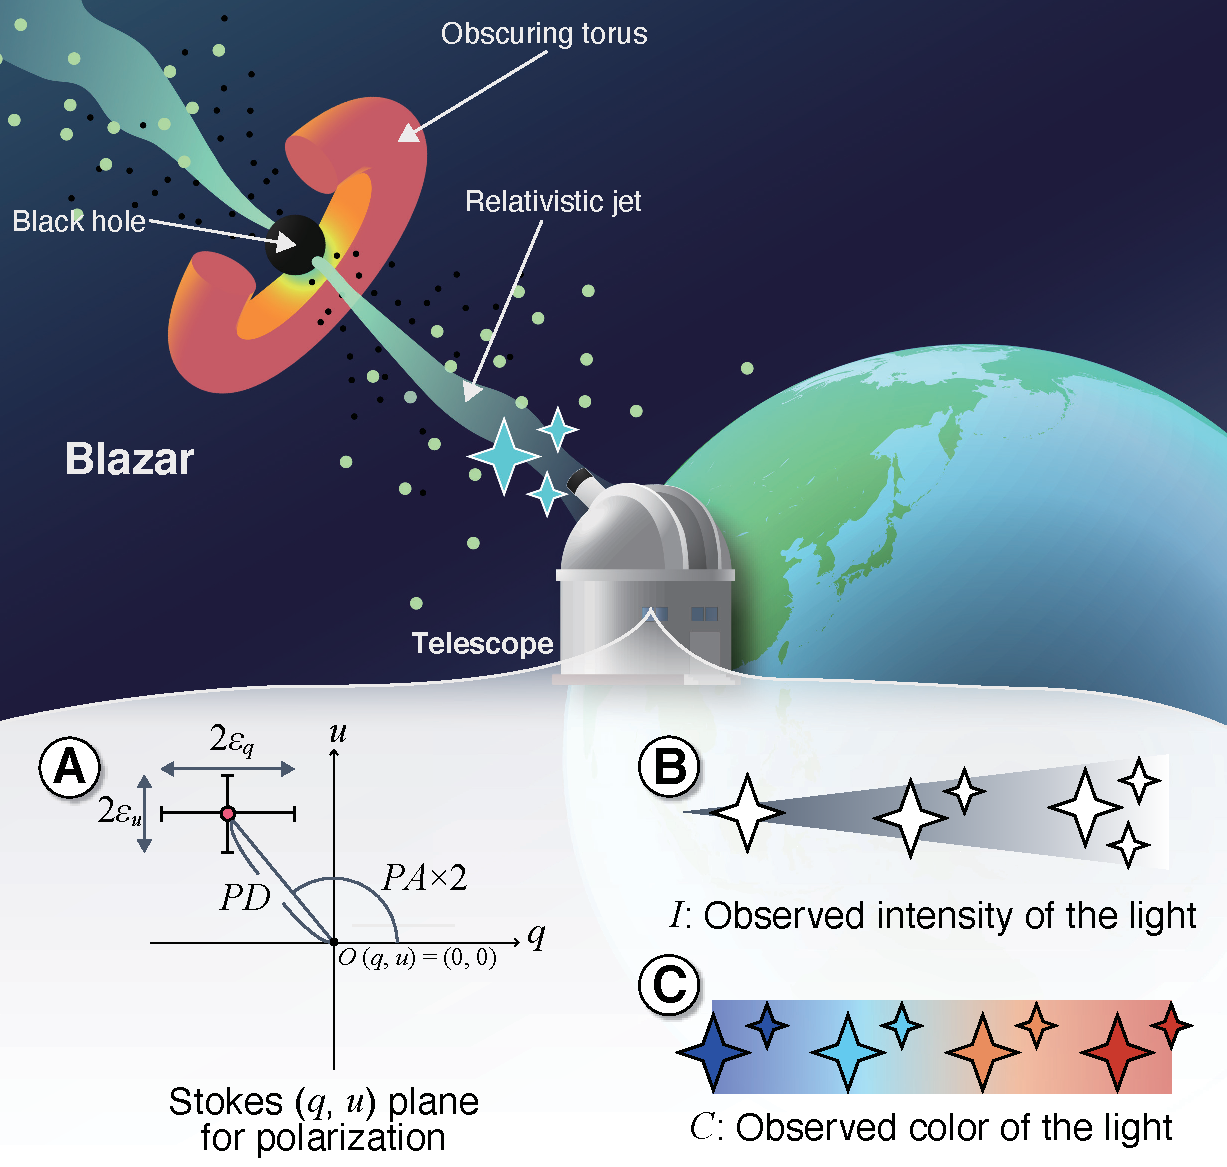
\includegraphics[width=.99\linewidth]{figures/blazar_final.pdf}
    \caption{An observed blazar and its features. A blazar's central black hole emits a relativistic jet toward the Earth.
        The telescope observes its light in terms of (A) polarization, (B) intensity, and (C) color.}
    \label{fig:blazar}
\end{figure}

\subsection{Goals and Visualization Tasks}\label{sec:domainGoalsandTasks}
We interviewed two astronomers at Hiroshima University, one at Stanford University, and four at Boston University to clarify the domain goals and visualization tasks.
The main objective of these astronomers is 
to quickly extract and analyze features in temporal variations of the observed polarization, intensity, and color that are occurring at multiple time intervals. 
TimeTubesX effectively supports the following four domain goals:

\noindent\textbf{G1--Enhance the reliability of blazar observations}. 
Datasets always contain missing data and observation errors. 
Astronomers need to assess whether what they have found is plausible by analyzing the length of missing data periods and the size of errors.

\noindent\textbf{G2--Identify flares and rotations}. 
Astronomers typically pay attention to time intervals with dynamic time variations,
such as flares and rotations.
The analysis of time intervals with such dynamic variations helps astronomers demystify jets' structures.

\noindent\textbf{G3--Locate recurring blazar behaviors}.
Besides well-known behaviors such as flares and rotations, 
recurring patterns or common features can also exist.
Thus, upon finding an interesting pattern or feature, 
astronomers want to locate other time intervals similar to it.

\noindent\textbf{G4--Explore time intervals validating a hypothesis of blazar behaviors}.
Through their analyses or experiences, astronomers sometimes make a hypothesis (e.g., that the flares of a blazar tend to co-occur with a specific polarization variation pattern). 
Astronomers need to address time intervals that might validate the hypothesis.

To attain these four goals, we have identified five visualization tasks that TimeTubesX should support:

\noindent\textbf{T1--Uncertainty-aware visualization.} 
Users should be able to perceive the reliability of data through visualizations. 

\noindent\textbf{T2--Analysis across datasets.} 
To compensate for missing data, 
the system must allow users to aggregate datasets for the same target from different sources.
Analyses across datasets should also be supported to address features that are common to multiple targets.

\noindent\textbf{T3--Analysis of dynamic variations.} 
Time intervals with drastic changes in a short time period and those with unusually large time variations should be automatically extracted.

\noindent\textbf{T4--Similarity analysis of a specific region/shape of interest and time intervals.} 
Users should be able to identify regions/shapes of interest (\emph{ROI}s/\emph{SOI}s) and search for similar time variation patterns at other time intervals without using complex query languages or parameter settings.

\noindent\textbf{T5--Fuzzy search for time intervals similar to a specific ROI/SOI.}
The system should provide not only exact matches between a ROI/SOI and time intervals but also fuzzy or approximate matches. 

To support \textbf{G1}, our previous work, TimeTubes~\cite{Fujishiro2018}, has already supported \textbf{T1} and \textbf{T2}.
Observation errors are encoded in the appearance of the 3D volumetric tube (\textbf{T1}).
An ellipsoidal snapshot and a white cruciform axis appear at each observation timestamp to distinguish missing data (\textbf{T1}).
Analysis across datasets (\textbf{T2}) is supported by visual data fusion, which allows users not only to aggregate multiple datasets for the same blazar but also to effectively compare multiple datasets for the same or a different blazar in a single visualization session.
In this paper, we mainly focus on feature and pattern detection methods to support the remaining three tasks (\textbf{T3}, \textbf{T4}, \textbf{T5}).
Consequently, we have designed an integrated visual analytics framework for blazar observations that supports all identified goals (\textbf{G1}--\textbf{G4}) and tasks (\textbf{T1}--\textbf{T5}).

\section{System Design\label{sec:systemDesign}}
In this section, we provide an overview of visual encoding for blazar data and the visual exploration framework of TimeTubesX.

\begin{figure}[tb]
    \begin{minipage}{0.34\linewidth}
        \centering
        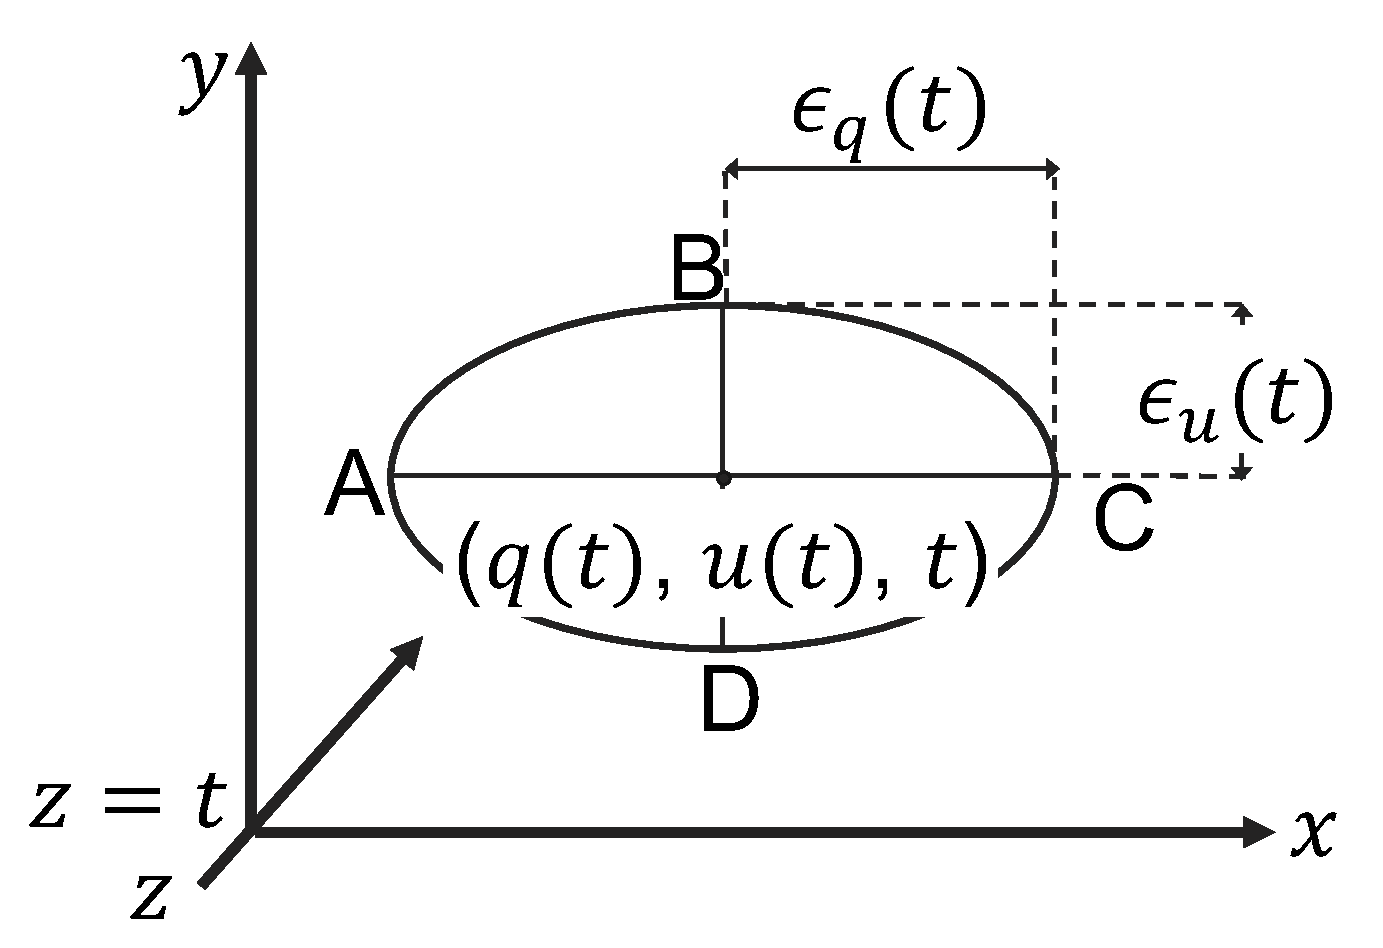
\includegraphics[width=.99\linewidth]{figures/howtoplot.pdf}
    \end{minipage}
    \begin{minipage}{0.26\linewidth}
        \centering
        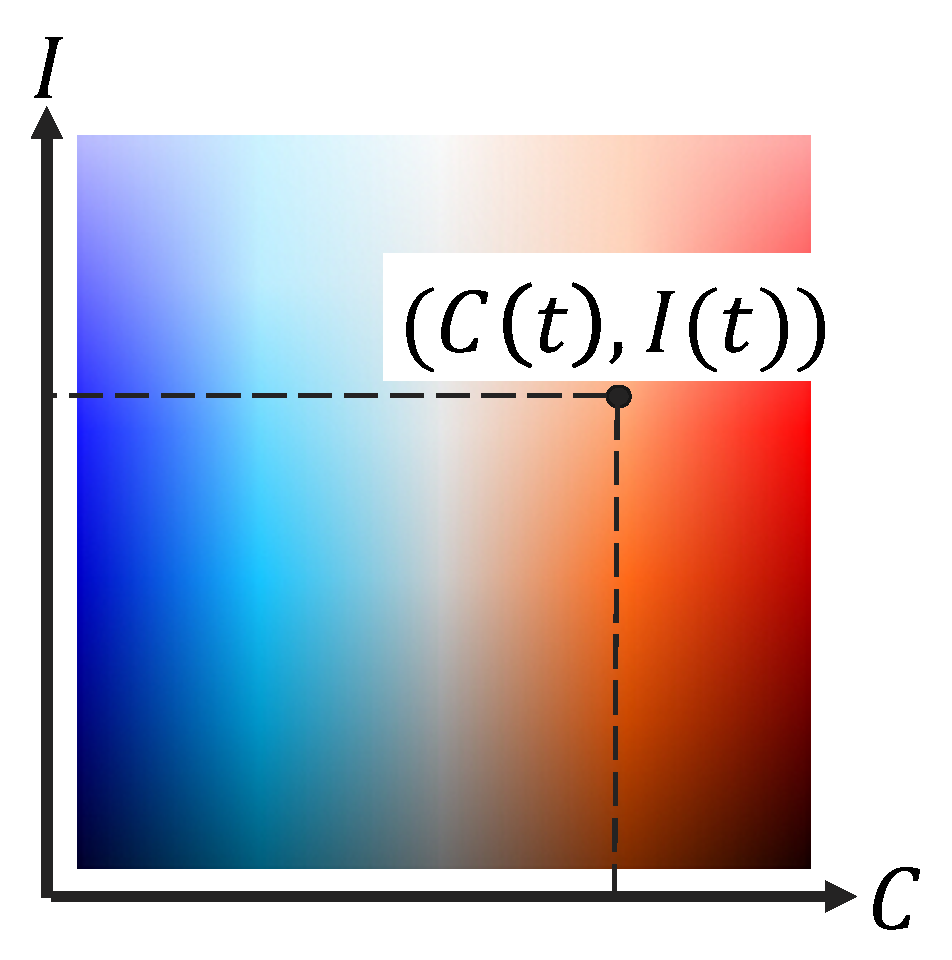
\includegraphics[width=.99\linewidth]{figures/colormap.pdf}
    \end{minipage}
    \begin{minipage}{0.36\linewidth}
        \centering
        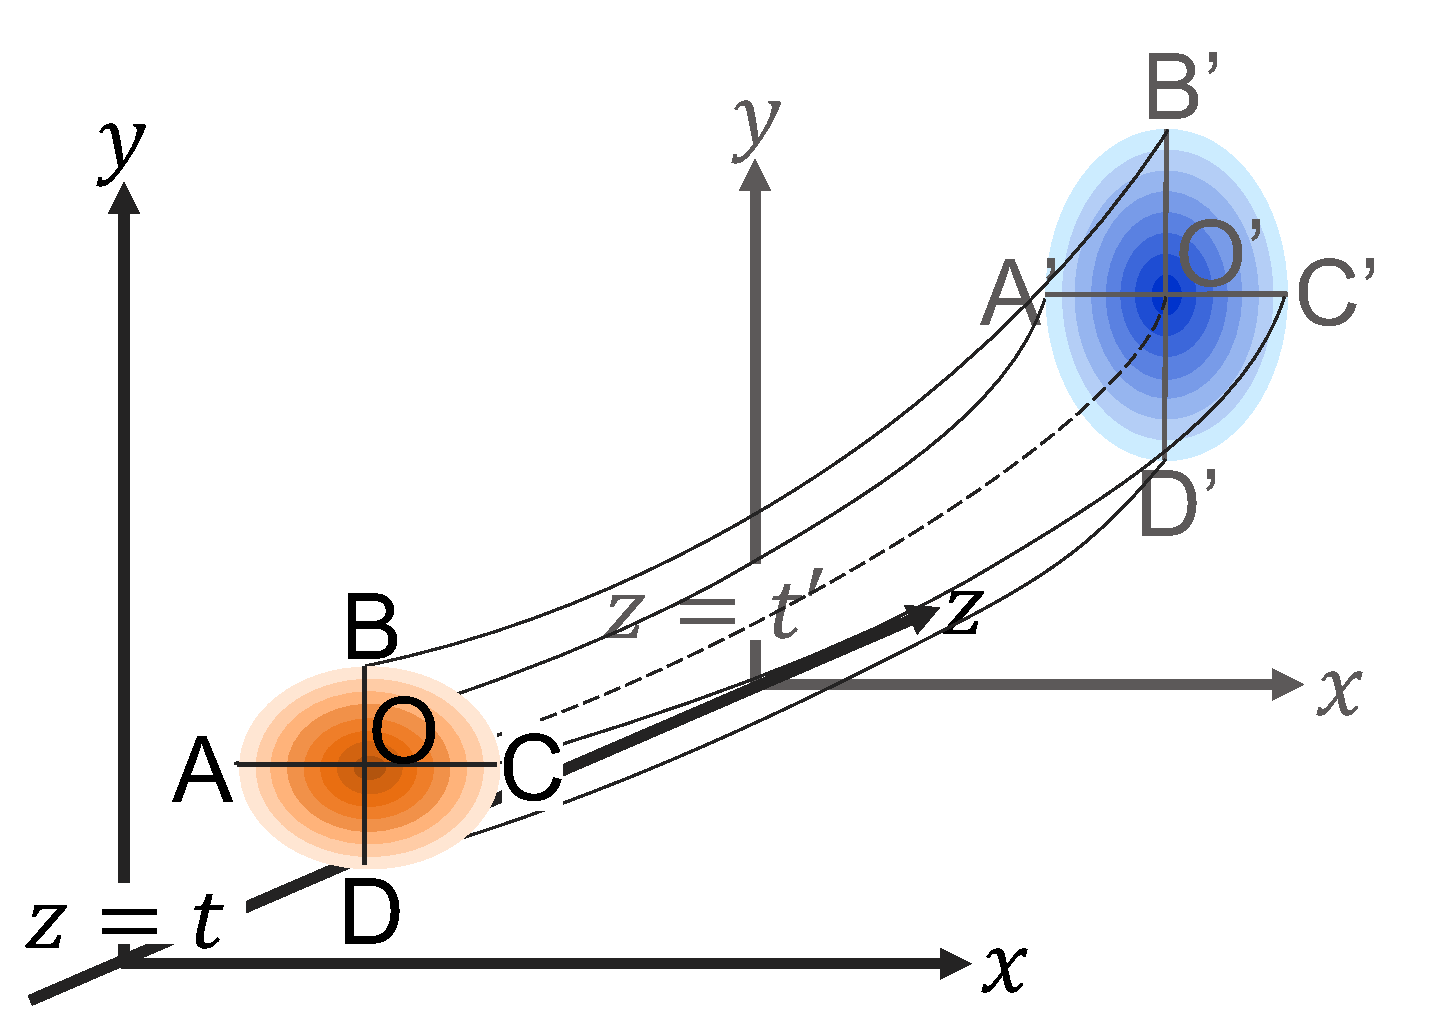
\includegraphics[width=.99\linewidth]{figures/howtotube.pdf}
    \end{minipage}
    \begin{minipage}{0.34\linewidth}
        \centering
        \footnotesize{\sf (a)}
        \end{minipage}
    \begin{minipage}{0.26\linewidth}
        \centering
        \footnotesize{\sf (b)}
    \end{minipage}
    \begin{minipage}{0.36\linewidth}
        \centering
        \footnotesize{\sf (c)}
    \end{minipage}
    \caption{Spatial mapping in the TimeTubes view. 
    (a)~Observation values of polarization decide the position and shape of an ellipse;
    (b)~observation values of intensity and color colorize the ellipse with reference to a colormap; and
    (c)~the neighboring ellipses are smoothly connected in chronological order to yield a tube shape.}
    \label{fig:howtoplot}
\end{figure}
\subsection{Visual Encoding for Blazar Data}\label{sec:VisualEncoding}
\begin{figure*}
    \centering
    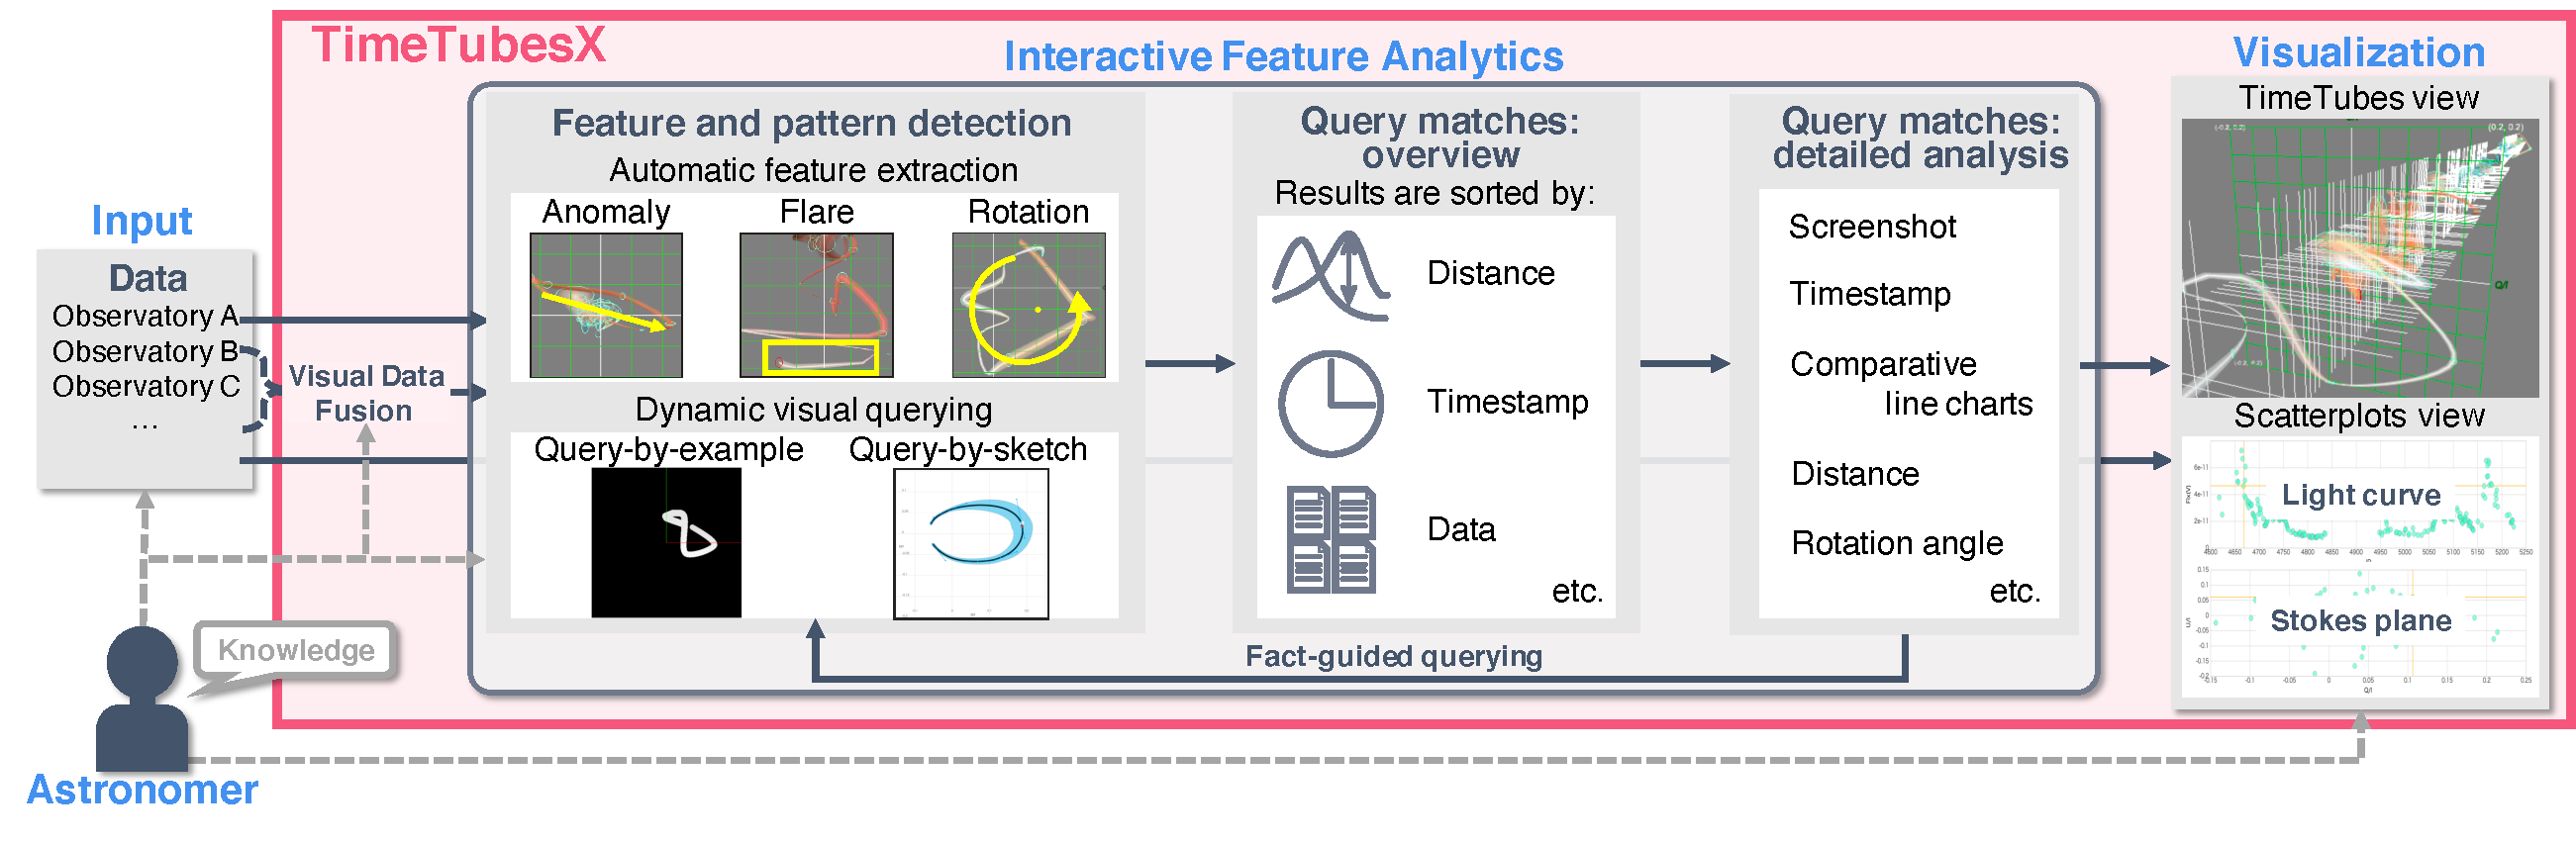
\includegraphics[width=.99\linewidth]{figures/workflowGray.pdf}
    \caption{The visual exploration framework of TimeTubesX. Users can load multiple datasets into a single exploration session through visual data fusion. (A)~Users specify a query to extract features of interest; (B)~query results are sorted by relevance; (C)~individual results can be analyzed in high detail and compared to each other; (D)~an extraction result can be re-used as an input for a new visual query; and (E)~users can visually explore the results in the TimeTubes and scatterplots views.}
    \label{fig:framework}
\end{figure*}
Astronomers have used three animated scatterplots with error bars to visualize their multi-dimensional, time-dependent observations (see the accompanying video): one for time variation of $I$, termed \textit{light curve}, another for the Stokes plane, and a third for the correlation between $I$ and $C$.
During the animation, individual observations are highlighted in red in order of observation.

Instead of animating multiple 2D scatterplots,
TimeTubesX expresses blazar observations as a single 3D volumetric tube. 
In the following part, we give an overview of the \emph{TimeTubes view}, which was originally proposed in our previous work~\cite{Fujishiro2018}.
The TimeTubes view allows users to see correlations and variations of variables over time at a glance, as illustrated in Fig.~\ref{fig:framework}~(E).
In the current version, users need to import .csv files with column names from their local environment into TimeTubesX.
We use a left-handed coordinate system to assign $q$ and $u$ to the $x$ and $y$ axes, respectively, and time $t$ to the $z$ axis.
We encode the polarization parameters ($q$, $u$, $\epsilon_q$, $\epsilon_u$) at each timestamp $t$ as an ellipse centered at the point $(x, y, z) = (q(t), u(t), t)$ with a width of $2\epsilon_q(t)$ and a height of $2\epsilon_u(t)$, as depicted in Fig.~\ref{fig:howtoplot}~(a). 
Therefore, the $x$--$y$ location of an ellipse indicates the polarization at a certain time stamp, while the size of the ellipse indicates the uncertainty of the measurement.
To properly render a 3D tube, we set the value range of the Stokes plane in the TimeTubes view with reference to the standard deviations of $q$ and $u$ in the datasets. 
In the current TimeTubes view, we empirically map a single day to a single voxel along the $z$ axis.
We colorize the ellipses according to $I(t)$ and $C(t)$ based on a user-defined 2D colormap (Fig.~\ref{fig:howtoplot}~(b)). 
The TimeTubes view connects neighboring ellipses in chronological order, using centripetal Catmull-Rom splines to form a 3D volumetric tube (Fig.~\ref{fig:howtoplot}~(c)). 
To further reflect the reliability of the observations, the TimeTubes view offers an adjustable opacity transfer function.
Multiple concentric tubes with different transparencies (i.e., higher opacities for inner tubes) compose a single tube that allows users to intuitively perceive the uncertainties of observations.
Specifically, a time interval with small errors looks like an opaque tube, whereas a time interval with large errors looks more semi-transparent and fuzzy.

Compared with the initial animated scatterplots,
the TimeTubes view provides more uncertainty-aware visual encoding for the analysis of blazar behaviors (\textbf{T1}).
Astronomers do not need to scrutinize multiple plots to understand correlations between variables
or move sliders back and forth 
to track time variations.


\subsection{Visual Exploration Framework\label{sec:approach}}
The design of TimeTubesX supports the visualization tasks outlined in Section~\ref{sec:domainGoalsandTasks}.
Fig.~\ref{fig:framework} illustrates our visual exploration framework.
%
The user workflow starts with visual data fusion~\cite{Fujishiro2018} to create a unified dataset for all subsequent analysis steps (\textbf{T2}).
For initial feature and pattern detection (A), users can either rely on automatic feature extraction methods for well-known blazar behaviors (\textbf{T3}) or define their own visual queries for a ROI/SOI (\textbf{T4}, \textbf{T5}).
The system ranks the results of the feature and pattern detection stage and shows the ranked matches (B).
Users can sort the results to, for instance, focus on time intervals that have the largest rotation or are the most similar to the input pattern.
The detailed analysis (C) helps users understand the behavior at the extracted time intervals and classify the results. 
To support iterative refinement of queries, users can build a follow-up query based on the result of a query (D). It allows users to find time intervals similar to the result (\textbf{T4}).
We call this \textit{fact-guided querying}, as it enables users to refine extraction results guided by previously detected features.
To analyze extracted time intervals in more detail, users can employ
the uncertainty-aware TimeTubes view (\textbf{T1}) as well as multiple linked scatterplots views (E).

\textsf{Interactive feature analysis interface.\ } 
Fig.~\ref{fig:UIFeatureExtraction} shows our feature and pattern detection user interface. 
The query specification panel (A) allows users 
to build a query with simple interactions either by selecting what to extract, picking a part of data as an input, or sketching time variation patterns.
After running a similarity search, 
TimeTubesX ranks and filters extraction results according to the parameters in panel (B),
and then it displays all relevant (i.e., non-filtered) extraction results as a collection of thumbnails in panel (E).
The distance distribution histogram in panel (B) helps users to further filter the number of results.
The timeline in panel (C) gives an overview of the temporal distribution of the results.
Users are able to recognize groups of results sharing identical data samples and temporal distribution features.
When selecting an individual thumbnail, TimeTubesX shows a detailed information on the corresponding result in panel (D), including exact timestamps and the distance between the query and the result.
To re-utilize the query, compare multiple query results, and share the query and their results with other users, 
TimeTubesX allows users to export and import queries and their results in the form of JSON files (a custom format for TimeTubesX).
When importing previous query results,
panel (F) shows a summary of the query used in the previous process and panel (C) shows another timeline for the imported query results.

Fig.~\ref{fig:querySpecificationPanel} shows the query specification panels for each mode of the feature and pattern detection.


To better demonstrate our feature and pattern detection methods, we will use a synthetic dataset (see Fig.~\ref{fig:synthesisData}) as a running example in Sections~\ref{sec:automaticExtraction} and \ref{sec:visualQuery}.
It contains four large peaks in $I$, as highlighted by orange diamonds in (a), three small red circular patterns on the Stokes plane in (b), three large green rotations , and three narrow/rough-edged blue patterns.

\begin{figure}[t]
    \begin{minipage}{\columnwidth}
        \begin{center}
            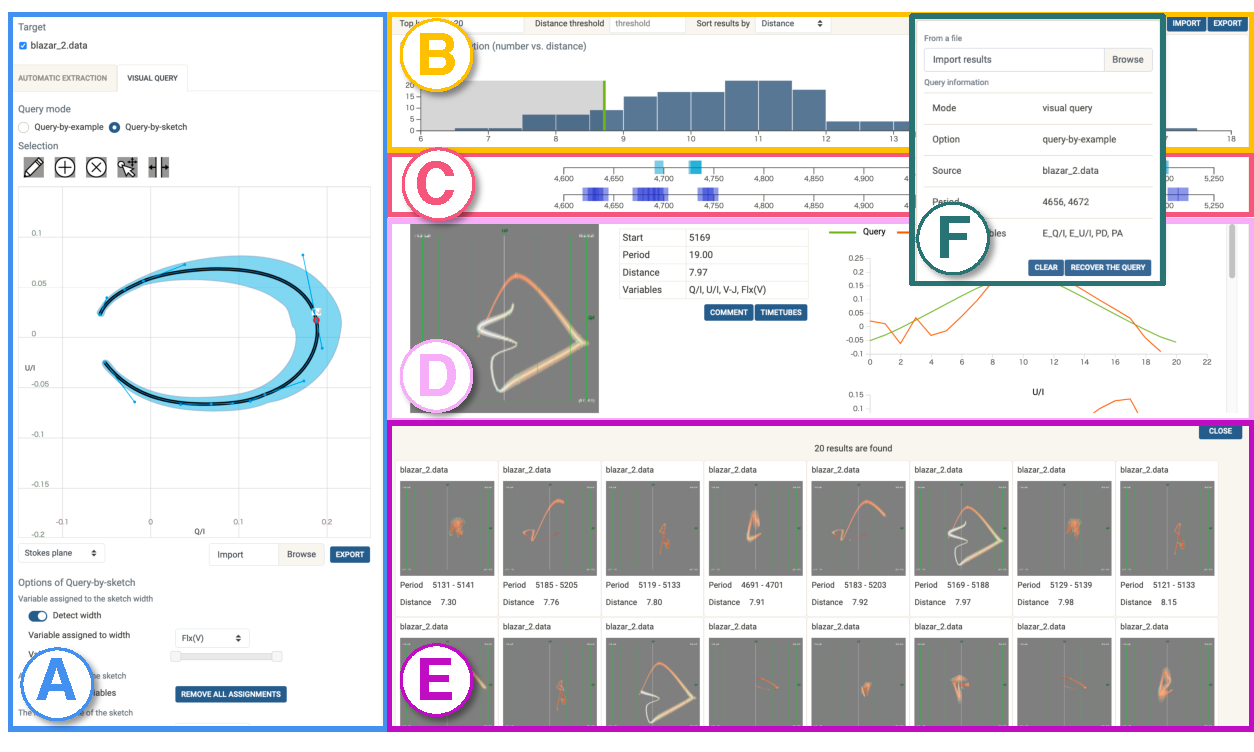
\includegraphics[width=.99\linewidth]{figures/GUI.pdf}
        \end{center}
        \begin{minipage}{\columnwidth}
        \caption{
        The user interface for interactive feature analysis. (A)~Query specification panel; (B)~parameters for ranking, filtering, and displaying extraction results and a histogram for the distribution of distances returned by the similarity search; (C)~timelines overviewing displayed extraction results; (D)~a detailed information panel for a selected result; (E)~a collection of thumbnails for extraction results; and (F)~summary of the imported previous extraction results.}
        \label{fig:UIFeatureExtraction}
        \end{minipage}
    \end{minipage}
\end{figure}
\begin{figure}[t]
    \begin{minipage}{\columnwidth}
        \begin{center}
            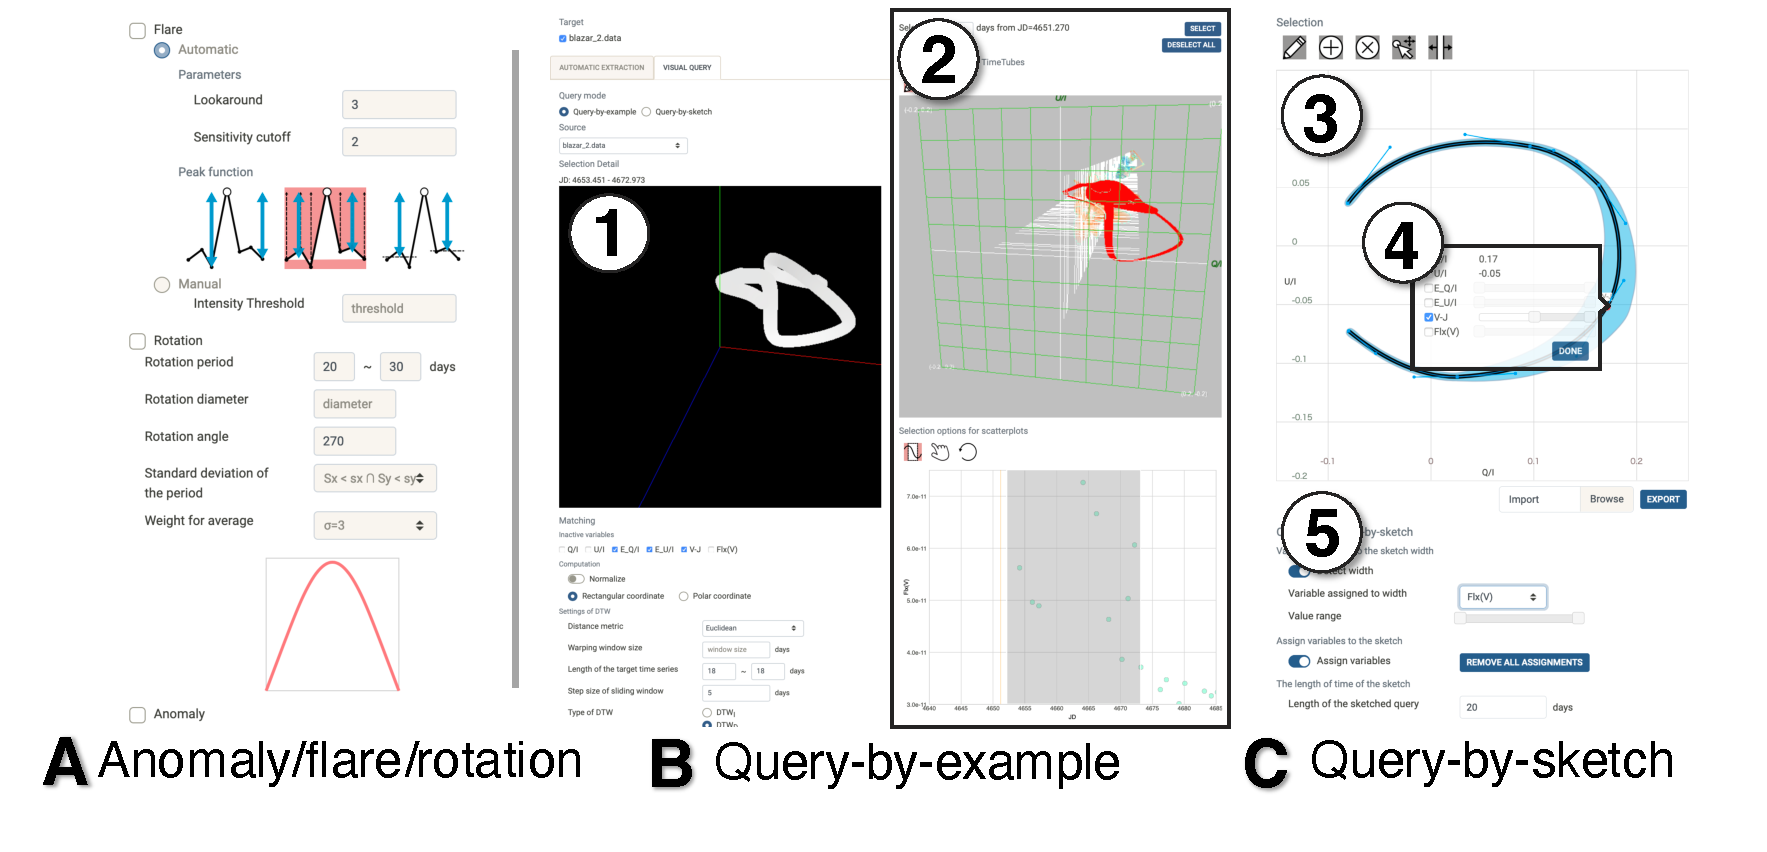
\includegraphics[width=.99\linewidth]{figures/QuerySpecificationPanel.pdf}
        \end{center}
        \begin{minipage}{\columnwidth}
        \caption{Query specification panels for feature and pattern detection methods. (A) Automatic feature extraction; (B) query-by-example, where users can check the selected time interval in a 3D tube view and further fine-tune query parameters (1) after selecting a time interval in the TimeTubes or scatterplots views (2);
         and (C) query-by-sketch, where users draw a SOI (3) and assign filtering constraints at each control point of the hand-drawn sketch (4) or adjust sketch pad settings (5).}
        \label{fig:querySpecificationPanel}
        \end{minipage}
    \end{minipage}
\end{figure}
\begin{figure}[t]
    \centering
    \vspace{3mm}
    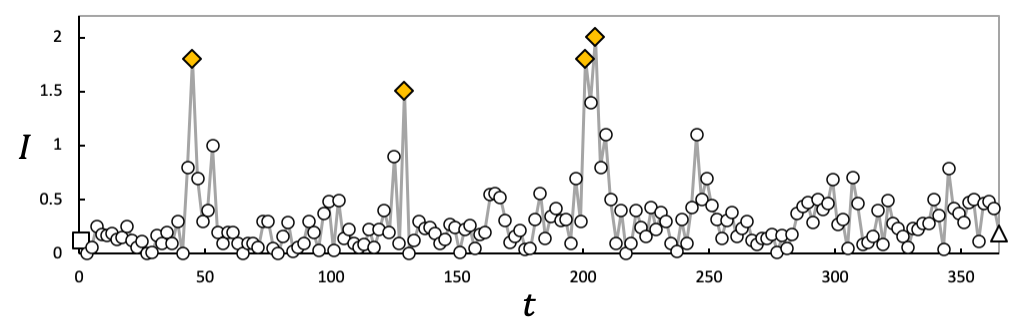
\includegraphics[width=.8\linewidth]{figures/synthesisDataLightCurveLabel_revised.png}\\
    \footnotesize{\sf (a) Light curve plot. The orange diamonds indicate peaks in the data.}\\
    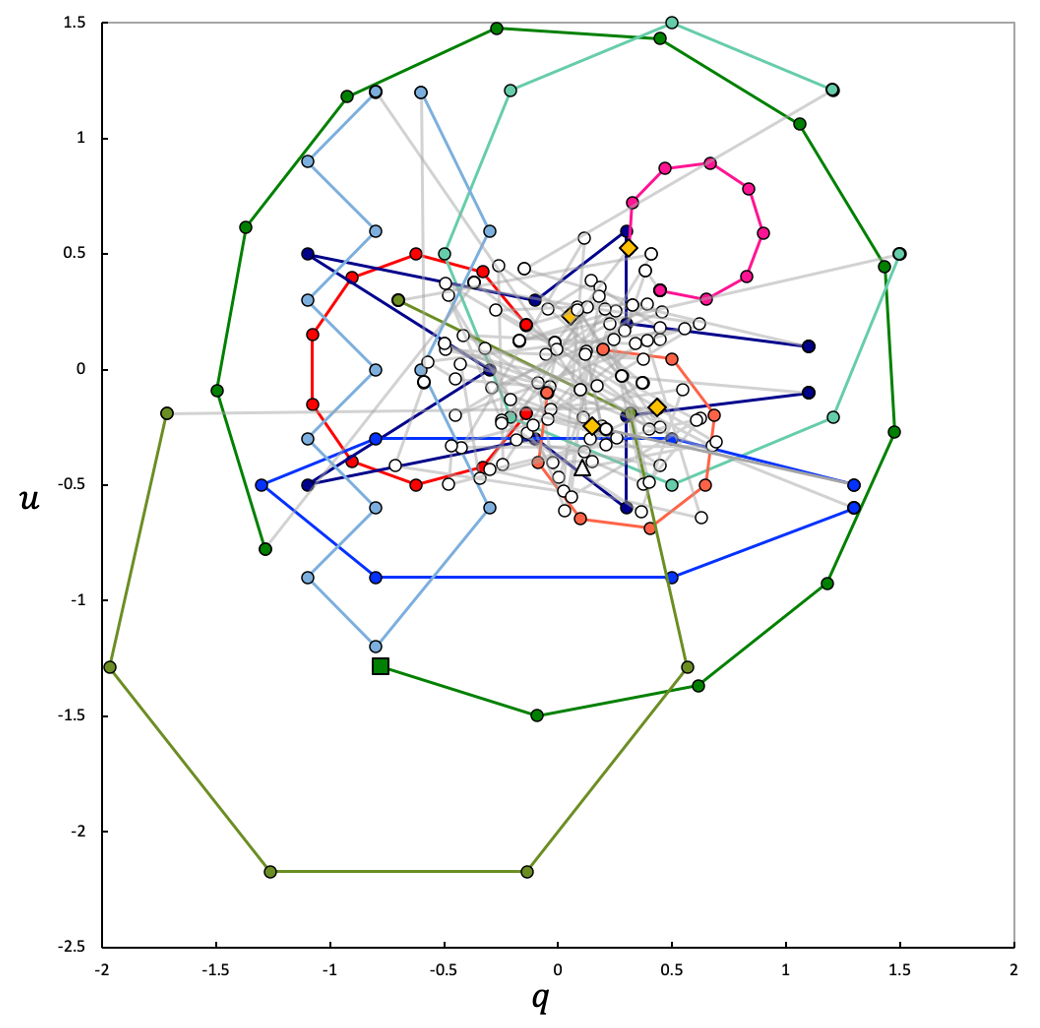
\includegraphics[width=.83\linewidth]{figures/synthesisDataStokesLabel_revised.png}\\
    \footnotesize{\sf (b) Stokes plane plot. The orange diamonds indicate the peaks in (a).}
    \caption{Conventional light curve plot and the Stokes plane for our synthetic dataset. The data has three small circular patterns (red), three large rotations (green), and three narrow/rough-edged patterns (blue) within 365 days. Data starts from the square mark and ends at the triangular mark.}
    \label{fig:synthesisData}
\end{figure}
\section{Automatic Feature Extraction}\label{sec:automaticExtraction}
Astronomers pay careful attention to unusual behaviors of blazars, such as flare and rotation.
As a first step to identify flares and rotations (\textbf{G2}),
we have implemented automatic feature extraction for the discovery and analysis of dynamic time variations (\textbf{T3}).
TimeTubesX automatically extracts three types of features: anomalies (Section~\ref{sec:anomalyDetection}), flares (Section~\ref{sec:flareDetection}), and rotations (Section~\ref{sec:rotationDetection}).
We have significantly improved the detection algorithms for flares and rotations compared with the ones in our previous work~\cite{Sawada2018} 
to identify flares more flexibly and detect rotations more accurately.
Fig.~\ref{fig:querySpecificationPanel} (A) shows the automatic feature extraction panel,
where users can select specific patterns and parameters for automatic feature extraction.
The node (A) in Fig.~\ref{fig:framework} shows example TimeTubes views for an anomaly, flare, and rotation.

\subsection{Anomaly Detection}\label{sec:anomalyDetection}
It is challenging for astronomers to manually identify time variations across multiple variables. 
We define data samples with drastic temporal changes in polarization, intensity, and color as \textit{anomalies}.
Tracking anomalies can result in identifying unusual time variations or presages of well-known behaviors, such as flares or rotations,
because observable blazar behaviors show a tendency to include these drastic variations.

The anomaly degree was defined in our previous work~\cite{Sawada2018} as the product of the change amount in polarization, intensity, and color per day:
\begin{equation*}
\begin{split}
  \int_t^{t + 1}\left|\frac{dPolar(t)}{dt}\right|\cdot\left|\frac{dI(t)}{dt}\right|\cdot\left|\frac{dC(t)}{dt}\right|dt,
  \label{eq:anomaly}
\end{split}
\end{equation*}
where $Polar(t)$ means the position of a data sample on the Stokes plane at time $t$, and $I(t)$ and $C(t)$ stand for intensity and color, respectively. 

\textsf{Experimental results.\ } Applying the anomaly detection to our synthetic data, 
data samples around extreme peaks (the orange diamonds in Fig.~\ref{fig:synthesisData}~(a)) and parts of dynamic rotations (the green plots in (b)) were highly ranked.


\subsection{Flare Detection}\label{sec:flareDetection}
Flares are defined as extreme peaks of brightness (i.e., emitted light intensity). 
Astronomers regard flares as one of the most important observed behaviors of blazars.
However, since there is no specific threshold value of $I$ to define a flare, 
they need to analyze the local temporal profile of $I$ to identify flares.
We have updated the flare detection methods used in our previous work~\cite{Sawada2018}
to detect relatively small local flares as well as globally large flares.
To that end, we utilize peak detection methods for time-series data~\cite{Palshikar2009} to extract flare candidates. 
Flare detection comprises the following two steps:
\begin{enumerate}[nosep, label=\textsl{Step \arabic*}:, ref=\textsl{Step \arabic*}, align=parleft, leftmargin=*]
    \item \textsl{Compute the spikiness score $S$ for each data sample}; \label{algo:flareSpikiness}
    \item \textsl{Filter out data samples with a globally small $S$}. \label{algo:flareFilter}
\end{enumerate}
TimeTubesX uses Equation~\ref{equ:S2} to compute the spikiness score $S$ for \ref{algo:flareSpikiness};
we tested multiple equations for $S$ and empirically found that the following one produces the best results:
\begin{eqnarray}
    S &=& \frac{\frac{\sum_{k=1}^{K}(x_i - x_{i - k})}{K} + \frac{\sum_{k=1}^{K}(x_i - x_{i + k})}{K}}{2}\label{equ:S2},
\end{eqnarray}
where $x_i$ denotes a data sample indexed as $i$ and $K$ denotes the number of neighbors that should be examined.
Equation~\ref{equ:S2} provides the average values of the averages of distances between $x_i$ and $K$ left neighbors and those between $x_i$ and $K$ right neighbors.
\ref{algo:flareFilter} retains only data samples that satisfy $S - \bar{S} > h \times \sigma_{S}$, 
where $\bar{S}$ and $\sigma_{S}$ denote the mean and standard deviation of all computed $S$ values for the dataset, respectively, 
and $h$ is a user-specified sensitivity threshold. 
The original algorithm~\cite{Palshikar2009} merges peaks that are close together into one, 
but we did not adopt this strategy
because astronomers are equally interested in small, individual flares and large, aggregated flares.

\begin{figure}[tb]
    \centering
    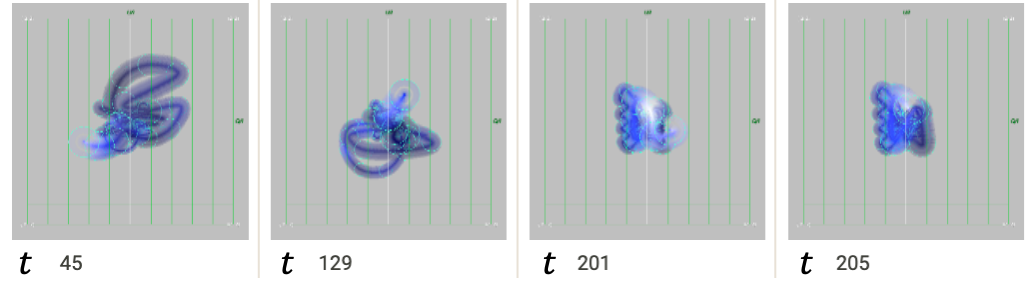
\includegraphics[width=.85\linewidth]{figures/flareDetectiondemodataResults.png}
    \caption{Flare detection results for our synthetic data. The results match the four red data samples in Fig.~\ref{fig:synthesisData}~(a).}
    \label{fig:flareDetection}
\end{figure}
\begin{figure}[tb]
    \centering
    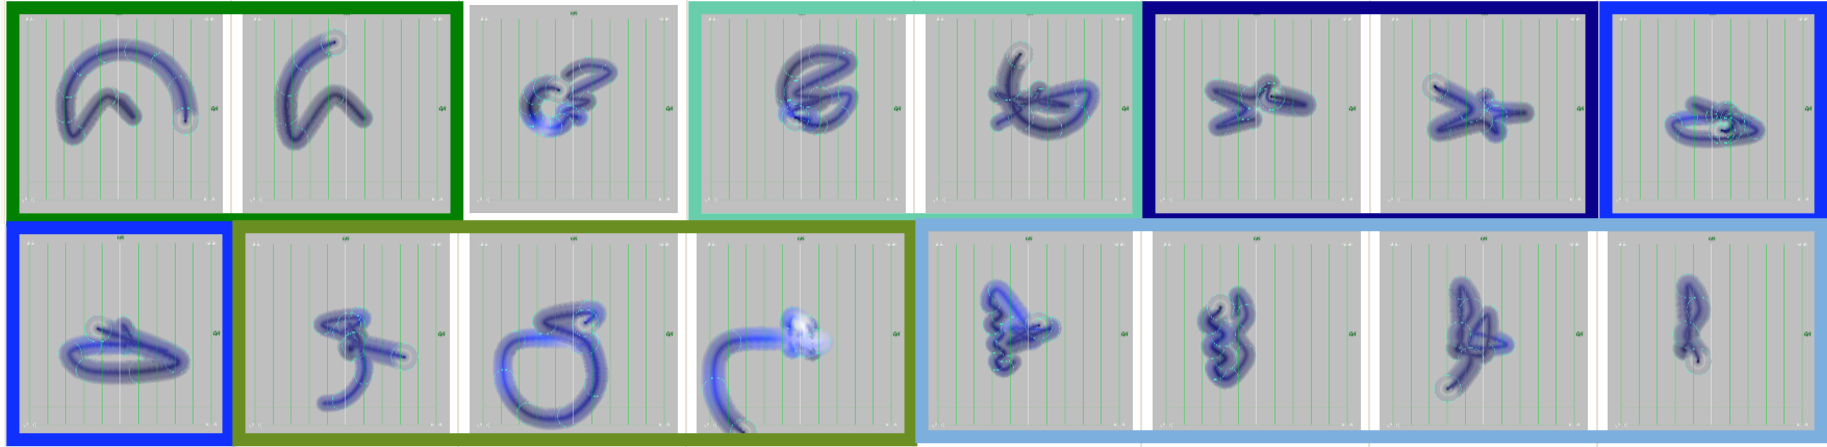
\includegraphics[width=\linewidth]{figures/rotationDetectiondemodataResultsOR.png}\\
    \footnotesize{\sf(a) Previous rotation detection method~\cite{Fujishiro2018}.}\\
    \vspace{5px}
    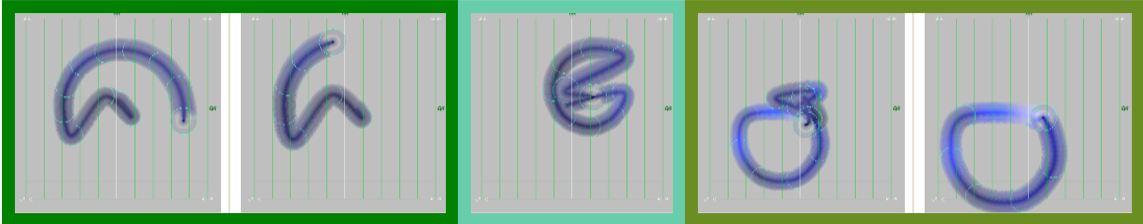
\includegraphics[width=.8\linewidth]{figures/rotationDetectiondemodataResults.png}\\
    \footnotesize{\sf(b) Our improved method.}
    \caption{Rotation detection results for our synthetic dataset in Fig.~\ref{fig:synthesisData}. 
        The outline color corresponds to the color in Fig.~\ref{fig:synthesisData}~(b).
        Our previous method detected narrow/rough-edged patterns and noise (blue), 
        whereas our improved method detected only large rotations (green).}
    \label{fig:rotationResults}
\end{figure}

\textsf{Experimental results.\ } We applied the flare detection method to our synthetic data.
We set $K$ and $h$ to 3 and 1, respectively.
Fig.~\ref{fig:flareDetection} presents the flare detection results.
The four data samples were detected as flares,
which completely coincide with the deliberately generated peaks that are highlighted in orange in Fig.~\ref{fig:synthesisData}~(a).

\subsection{Rotation Detection}\label{sec:rotationDetection}
Polarization rotation is another important observed behavior of blazars. 
Astronomers do not yet agree on whether rotation is an actual feature or just a result of random variations of polarization.
To validate their hypotheses, they scrutinize correlations between polarization and other properties at the time interval.
They typically have been analyzing the time variation of $PA$ to identify rotations~\cite{Ikejiri2011, Uemura2017},
but the rotation center will not be located at the origin of the Stokes plane ($(q, u) = (0, 0)$) when there are multiple polarized components in the sky.
Thus, estimating a rotation only through $PA$ may not allow astronomers to adequately understand its behavior.
Our rotation detection is capable of addressing any rotations regardless of the position of the rotation center.

We use a sliding window approach that allows users to manually define the length of the time interval for the sliding window. Based on feedback from astronomers~\cite{Sasada2012}, we set the default window size to be between three and four weeks.

The computation of the rotation angle is divided into the following seven steps:
\begin{enumerate}[nosep, label=\textsl{Step \arabic*}:, ref=\textsl{Step \arabic*}, align=parleft, leftmargin=*]
    \item \textsl{Compute the weighted means ($\overline{q}, \overline{u}$) of $q$ and $u$ at the time interval};\label{algo:rotationMean}
    \item \textsl{Compute the standard deviations ($\sigma_{q}, \sigma_{u}$) of $q$ and $u$ at the time interval}; \label{algo:rotationStd}
    \item \textsl{Convert the rectangular coordinates ($q-u$ domain) to polar coordinates ($r - \theta$ domain) with its origin shifted to $(\overline{q}, \overline{u})$}; \label{algo:rotationPolar}
    \item \textsl{Filter out time intervals whose $\sigma_{q}$ or $\sigma_{u}$ is smaller than the standard deviations of the entire dataset}; \label{algo:rotationFilter}
    \item \textsl{Compute the difference ($\theta_{\rm diff}$) of the $\theta$'s of two consecutive data samples}; \label{algo:rotationDiff}
    \item \textsl{Sum $\theta_{\rm diff}$'s to yield $\theta_{\rm sum}$}; \label{algo:rotationSum}
    \item \textsl{Check whether $\theta_{\rm sum}$ is larger than the user-specified threshold for the total rotation angle}. \label{algo:rotationThreshold}
\end{enumerate}
We regard $\overline{q}$ and $\overline{u}$ as a rotation center. 
To avoid misleading effects of outliers and unexpected values at the edges of a time interval,
smaller weights are assigned to both ends of the time interval according to a Gaussian distribution at \ref{algo:rotationMean}.
Note that users are allowed to adjust these weight ratios.
To avoid misclassifying time intervals with large $q$ or $u$ variance and unlike rotations as rotation candidates,
we have improved upon our previous rotation detection method~\cite{Sawada2018} on the basis of feedback from two astronomers at Hiroshima University~\cite{Huang2019}.
To detect only large rotations, 
our new method is able to filter out time intervals in which \textbf{either} $\sigma_{q}$ \textbf{or} $ \sigma_{u}$ is smaller than the standard deviation of the entire dataset. 
Note that this and other provided filtering constraints also allow for discovery of small or narrow rotations, such as the red and blue patterns in Fig.~\ref{fig:synthesisData}~(b).
At \ref{algo:rotationDiff}, we cannot compute $\theta_{\rm diff}$ simply by subtracting the $\theta$'s of consecutive observations 
due to the range constraint on $\theta_{\rm diff}$ (i.e., $\theta_{\rm diff} \in [0, 2\pi]$). 
For example, when two successive data samples are located in the first and fourth quadrant of the Stokes plane, 
we need to consider whether to take the clockwise or counterclockwise direction as $\theta_{\rm diff}$. 
We determine the rotation direction 
by checking increasing/decreasing tendency in $\theta$'s with exponential smoothing~\cite{Brown1956}.
It forecasts the next value according to past observations by assigning larger weights to more recent observations.
In this way, it addresses the uncertainty about the rotation direction and make results more feasible (\textbf{T1}).
We estimate the variation trend of $\theta$ and
then define the angle in the predicted rotation direction as $\theta_{\rm diff}$.
Users can set an arbitrary angle as a threshold parameter at \ref{algo:rotationThreshold}.

\textsf{Experimental results.\ } To compare our novel algorithm with the previous rotation detection algorithm~\cite{Sawada2018}, we applied both to our synthetic data.
As the results in Fig.~\ref{fig:rotationResults}~(a) show, 
the previous algorithm detected not only large rotations (green patterns in Fig.~\ref{fig:synthesisData}~(b)) but also narrow or rough-edged patterns (blue).
The improved algorithm more accurately detected only time intervals in which the polarization values dynamically rotate (green), as shown in Fig.~\ref{fig:rotationResults}~(b).
\section{Dynamic Visual Querying}\label{sec:visualQuery}
To facilitate astronomers' discovery of time intervals similar to a ROI/SOI (\textbf{G3}) or those validating specific hypotheses (\textbf{G4}), 
TimeTubesX provides two different user-initiative visual query interfaces: query-by-example (QBE) and query-by-sketch (QBS).
Both are designed to help users identify similar patterns of interest (\textbf{T4}), and our matching algorithm allows for a fuzzy search (\textbf{T5}).

\subsection{Query-by-Example}\label{sec:QBE}
While the TimeTubes view helps users analyze time variations,
it remains challenging for users to build queries for multi-dimensional, time-dependent data.
Our QBE interface allows users to specify a notable behavior as a ROI with simple interactions through the TimeTubes or scatterplots views.
Users can pick a part of time-series data as an input for a query as well as flexibly select specific variables that should be queried about to reflect their intentions. 
This allows users to easily and intuitively search long-term datasets for interesting patterns with minimal required user inputs.

Fig.~\ref{fig:querySpecificationPanel} (B) shows our QBE interface.
To facilitate visual verification by users, a time interval selected through the TimeTubes or scatterplots views in (2, red highlight) is automatically extracted and displayed in the query panel (1).
After selecting the initial time interval, users can then fine-tune and adjust their query by selecting the variables that should be queried about. 
This is crucial for effective support of queries on multi-dimensional data.
Based on the selected variables, 
our system interactively updates the appearance of the 3D tube for the selected time interval in (1), visually encoding only currently selected variables.
For example, when users remove the variable $C$ from the query, the tube loses color variation and becomes a gray tube, as shown in (1).
After defining the query, users can adjust the main parameters (e.g., normalization and polar coordinates options) for our matching algorithm (see Section~\ref{sec:matchingAlgorithm}). 

\textsf{Experimental results.\ } We verified the effectiveness of our QBE method using our synthetic data.
The red circular patterns in Fig.~\ref{fig:synthesisData}~(b) have a similar shape but different time lengths, scales, or locations in the Stokes plane.
We used the leftmost red time interval in (b) as an input query, as shown in Fig.~\ref{fig:QBEDemodata}~(a).
We selected $q$ and $u$ as active variables and used the normalization and polar coordinates options to detect time intervals with different scales or different positions.
The length of the target time interval was set to 5 to 20 days.
We used $\rm{DTW}_{\rm D}$ as a distance function.
Note that we detail the options and parameters related to the matching process in Section~\ref{sec:matchingAlgorithm}.
Fig.~\ref{fig:QBEDemodata}~(b) shows the top three results of our QBE in (a).
The color of the rectangles corresponds to those used in Fig.~\ref{fig:synthesisData}~(b).
We were able to detect all time intervals with a similar shape in our synthetic dataset.
Note that the time interval specified for the query itself is omitted from the results.

\begin{figure}[tb]
    \centering
    \begin{minipage}{0.24\linewidth}
        \centering
        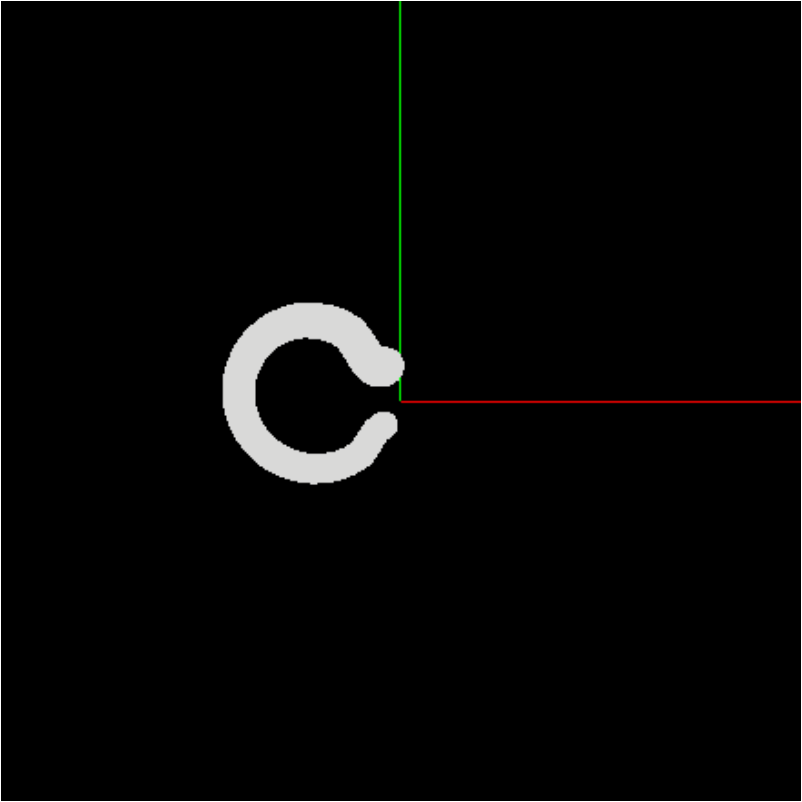
\includegraphics[width=.99\linewidth]{figures/QBE.png}
        \footnotesize{\sf (a)~Query.}
    \end{minipage}
    \begin{minipage}{0.75\linewidth}
        \centering
        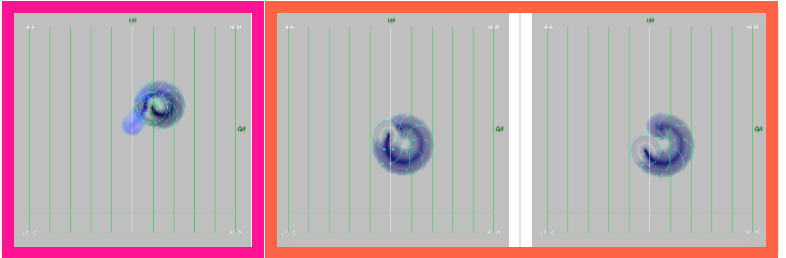
\includegraphics[width=.99\linewidth]{figures/QBEdemodataResults_revised.png}
        \footnotesize{\sf(b)~Results for the query in (a).}
    \end{minipage}
    \caption{QBE for our synthetic dataset in Fig.~\ref{fig:synthesisData}. 
        We chose the time interval with a small circular pattern (the leftmost red pattern in Fig.~\ref{fig:synthesisData}~(b)) for a query in (a). 
        Our method precisely extracted other time intervals with small circular patterns (the two red patterns from the right in Fig.~\ref{fig:synthesisData}~(b)).
        The outline color corresponds to the color in Fig.~\ref{fig:synthesisData}~(b).}
    \label{fig:QBEDemodata}
\end{figure}
\subsection{Query-by-Sketch}\label{sec:QBS}
TimeTubesX also allows users to query their data by manually drawing time variation patterns onto a 2D sketch interface.
Our QBS interface provides an intuitive and accessible way for users to specify patterns for multi-dimensional, semi-structured, time-dependent blazar datasets and validate their high-level hypotheses.
Rouxel et al.~\cite{Rouxel2014} state that an input trajectory by analog gestures is characterized by three dimensions: space, time, and force.
To realize intuitive interactions, 
we use space to determine the $x$ and $y$ positions of the stroke
and use either drawing speed or drawing pressure to define the stroke width 
so that users can describe time variations of multiple dimensions simultaneously.
Using the drawing speed option, the longer a cursor stays on a single point, the wider the curve at the point becomes.
To take into account other variables that are not described in sketching gestures, 
our QBS interface allows users to assign filtering constraints for each variable.
Thus, a sketch-based query for multi-dimensional, semi-structured, time-dependent data can be built with a single gesture
without sketching time variation patterns several times.

Fig.~\ref{fig:querySpecificationPanel} (C) shows the QBS query specification panel.
First, users define which variables are assigned to the $x$ and $y$ axes of the sketch pad and the stroke width (see panel (5)).
Second, they sketch a time variation pattern on a 2D sketch pad UI (3),
where the stroke is shown in black and its width is shown in blue.
Afterward, our system automatically beautifies the input stroke by fitting it to a cubic Bezier curve with as few segments as possible by using the \texttt{\small simplify} method in Paper.js~\cite{paper_framework}.
After their initial drawing, users can further adjust the sketch
by adding, removing, or moving control points or by changing the stroke width.
Users are also allowed to assign filtering constraints to each of the control points on the stroke, as shown in part (4).
They can define value ranges for each variable at the control point, which the algorithm will subsequently use when evaluating the query.

\begin{figure}[tb]
    \centering
    \begin{minipage}{0.49\linewidth}
        \centering
        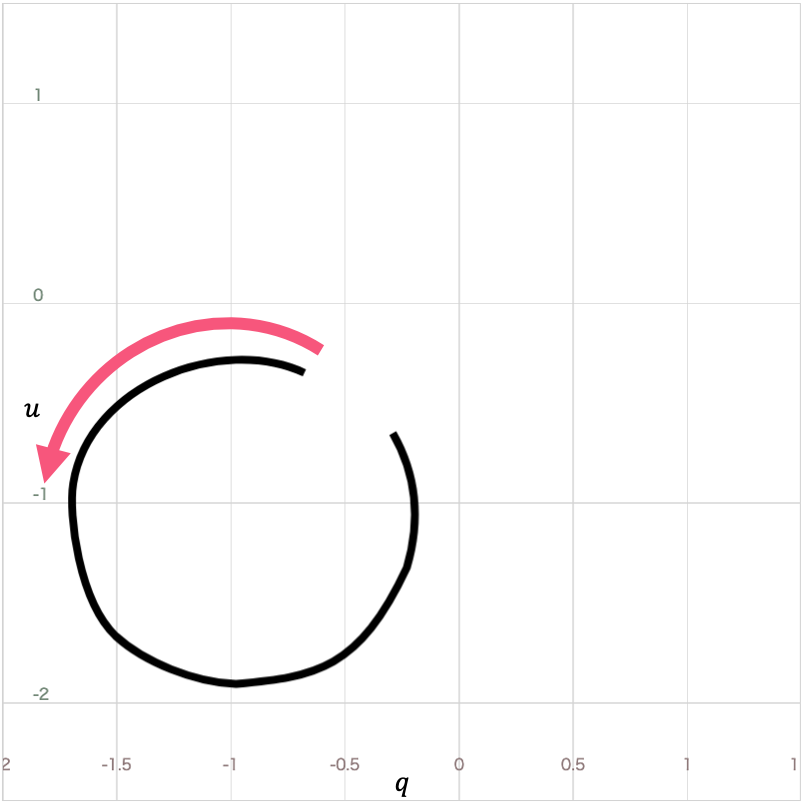
\includegraphics[width=.9\linewidth]{figures/QBSSketchwithoutWidth.png}
    \end{minipage}
    \begin{minipage}{0.49\linewidth}
        \centering
        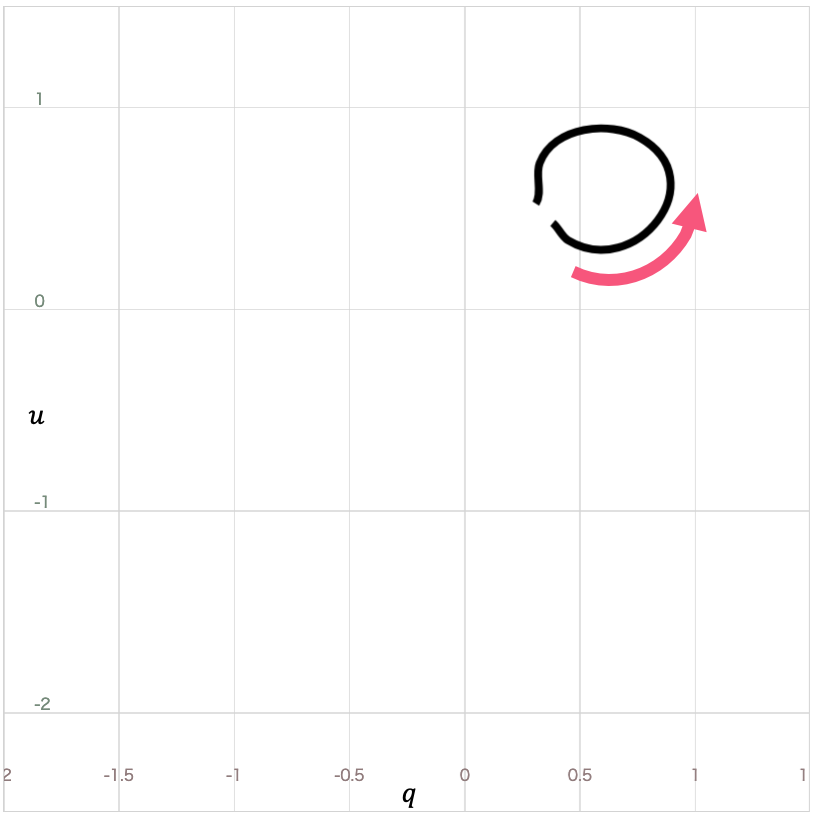
\includegraphics[width=.9\linewidth]{figures/QBSResultQuerywithoutWidth.png}
    \end{minipage}
    \begin{minipage}{0.49\linewidth}
        \centering
        \footnotesize{\sf (a)~A hand-drawn sketch query for a small circular pattern.}
    \end{minipage}
    \begin{minipage}{0.49\linewidth}
        \centering
        \footnotesize{\sf (b)~A sketch based on the upper left result in (c). 
        }
    \end{minipage}
    \begin{minipage}{0.49\linewidth}
        \centering
        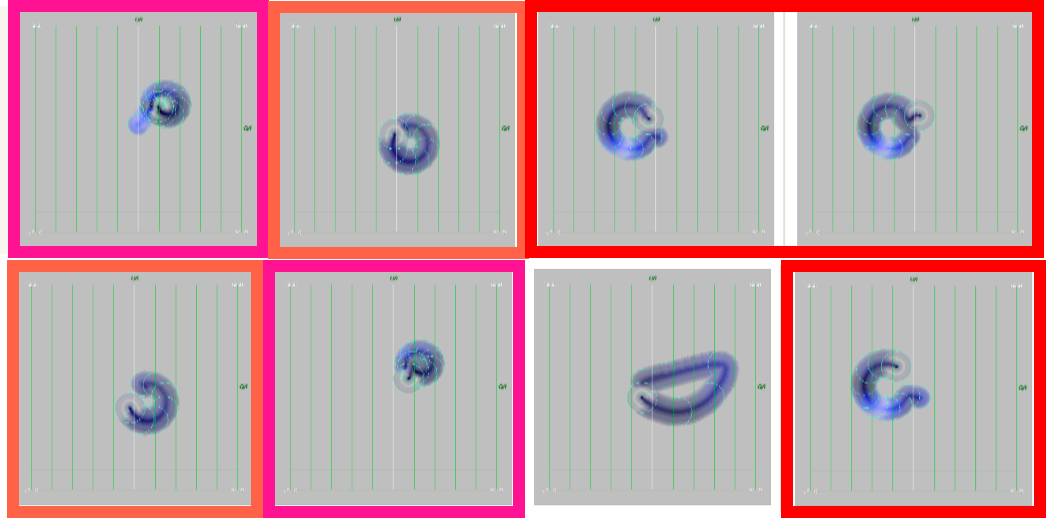
\includegraphics[width=.99\linewidth]{figures/QBSResultsHanddrawn_revised.png}\\
        \footnotesize{\sf (c)~Results for the query in (a).}
    \end{minipage}
    \begin{minipage}{0.49\linewidth}
        \centering
        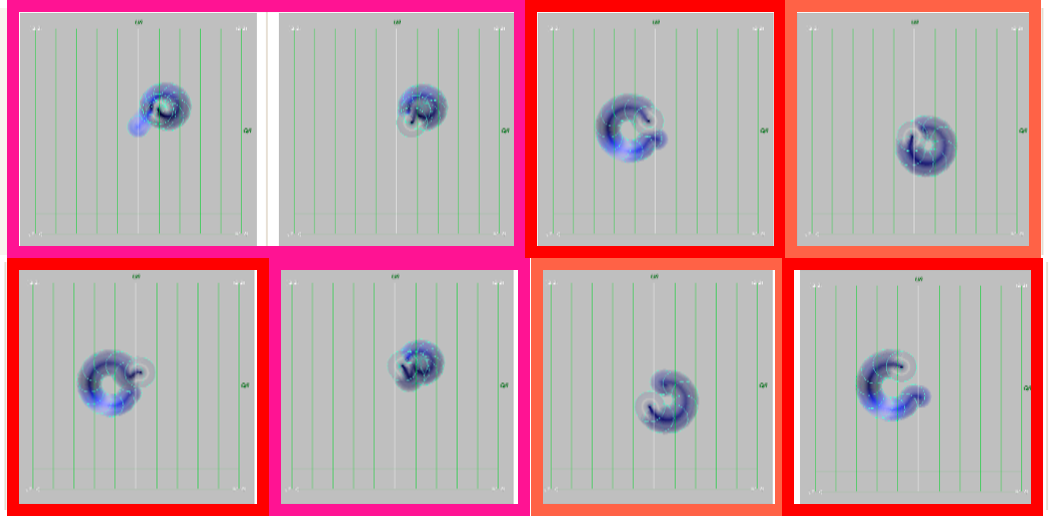
\includegraphics[width=.99\linewidth]{figures/QBSResultsResultQuery_revised.png}\\
        \footnotesize{\sf (d)~Results for the query in (b).}
    \end{minipage}
    \caption{QBS results for our synthetic dataset in Fig.~\ref{fig:synthesisData}.
        On the basis of a hand-drawn sketch in (a), an unexpected result is highly ranked (white outline) in (c). 
        With a sketch based on actual data values (b), no unexpected results appear, as illustrated in (d).
        }
    \label{fig:QBSDemodata}
\end{figure}
\textsf{Experimental results.\ } We evaluated the effectiveness of our QBS method using our synthetic data.
First, we sketched a pattern shown in Fig.~\ref{fig:QBSDemodata}~(a) to extract time intervals with small circular patterns.
The sketch pad plane corresponds to the Stokes plane, and for simplicity, the stroke width is not used.
To detect time intervals with a similar shape but different positions or scales, we used the normalization and polar coordinates options.
Fig.~\ref{fig:QBSDemodata}~(c) shows the top eight results for our QBS in (a).
The outline color of each thumbnails matches the color of the corresponding pattern in Fig.~\ref{fig:synthesisData}~(b).
All three time intervals highlighted in red in Fig.~\ref{fig:synthesisData}~(b) were precisely extracted.
However, an unexpected result (i.e., the thumbnail with white outline in Fig.~\ref{fig:synthesisData}~(c)) was highly ranked as a candidate similar to the input sketch due to the ambiguities of the hand-drawn sketch.
We address this problem by incorporating fact-guided querying (see Section~\ref{sec:factDrivenQuerying}). 

\subsection{Query Matching Algorithm}\label{sec:matchingAlgorithm}
There are many different methods for computing the distance between two time series, such as Euclidean distance, uniform scaling, and dynamic time warping (DTW)~\cite{Berndt1994}.
TimeTubesX uses DTW
because it aligns two time series elastically and thus supports the comparison of time series with different lengths.
Additionally, it can compute the distance between two time series that are similar but locally out of phase.
%more intuitively even if they are out of phase in the time direction. 
According to Eichmann and Zgraggen~\cite{Eichmann2015}, the DTW similarity measurement seems to most closely match human perception.
There are multiple solutions for dealing with multi-dimensional data in DTW. 
TimeTubesX implements two options, ${\rm DTW}_{\rm I}$ (independent) and ${\rm DTW}_{\rm D}$ (dependent), both of which are based on the work of Shokoohi-Yekta et al.~\cite{Shokoohi-Yekta2015}.

${\rm DTW}_{\rm I}$ computes the distance between two time series for each dimension of the data separately. 
In the final step, it adds up all the individual distances to produce the final distance measure.
Consequently, this approach focuses more on the similarity of each dimension and less on correlations between different dimensions.
${\rm DTW}_{\rm D}$, on the other hand, computes the distance between two data samples directly over all dimensions (i.e., as Euclidean distance in $n$-dimensional space).
Therefore, this method focuses more on correlations among the different dimensions of a time series and less on the similarities of individual dimensions. 
By default, our system uses ${\rm DTW}_{\rm D}$ because correlations among variables are important for blazar behavior analysis.
Readers are recommended to consult \cite[Fig. 1]{Shokoohi-Yekta2015} for comprehensive illustrations of ${\rm DTW}_{\rm I}$ and ${\rm DTW}_{\rm D}$.
We use a sliding window approach in our matching algorithm.
Users can set the window size and the step size of the sliding window and also set a constraint on the largest allowed temporal shift (i.e., warping window size)
in the process of finding the best alignment between the query and time series.
Users can specify these parameters at the bottom of the query specification panel in Fig.~\ref{fig:UIFeatureExtraction}~(A).
Note that multiple time intervals with different lengths but that include the same data samples can be presented in the extraction results (see Fig.~\ref{fig:QBEDemodata} and Fig.~\ref{fig:QBSDemodata}~(c) and (d)).
The timelines in Fig.~\ref{fig:UIFeatureExtraction}~(C) help users recognize such time intervals. 

Normalization and polar coordinates options enable a fuzzy pattern search.
The normalization option instructs the system to normalize a query and time intervals into the range of $[0, 1]$.
Subsequently, the pattern search places great significance on the shape of the time variations, whereas the actual value ranges will be ignored.
With the polar coordinates option, 
$q(t)$ and $u(t)$ are converted into polar coordinates ($r-\theta$ domain) before computing similarities.
Subsequently, the pattern search with the normalization and polar coordinates options will also be able to extract patterns rotating around the origin of the Stoke plane.

\subsection{Fact-Guided Querying}\label{sec:factDrivenQuerying}
To support quick and iterative query refinement, TimeTubesX allows users to re-utilize individual extraction results as an input for follow-up queries, a process we have termed \emph{fact-guided querying}.
By iteratively updating a query, users can, in a step-by-step manner, identify more observable time intervals that reflect their intentions.
Therefore, fact-guided querying contributes immensely to drilling down into data as a part of the visual exploration framework of TimeTubesX in Fig.~\ref{fig:framework}.
In QBE, users can switch variables used in the matching process and modify the time range of the query, while in QBS, users can adjust the scale, shape, and axis of the input query or add further filtering constraints.
Thus, fact-guided querying helps users perform further pattern searches based on a time interval of interest found in the previous process or create a sketch-based query from references to actual data measurements instead of from a blank sketch pad.

Our system allows users to build a fact-guided query with simple interactions by, for example, dragging an extraction result either into the QBE interface (part (2) in Fig.~\ref{fig:querySpecificationPanel}~(B)) or into the sketch pad of the QBS interface (part (3) in Fig.~\ref{fig:querySpecificationPanel}~(C)).

\textsf{Experimental results.\ } We confirmed the usefulness of the fact-guided querying approach with our synthetic data.
As discussed in Section~\ref{sec:QBS}, 
hand-drawn sketch queries, such as Fig.~\ref{fig:QBSDemodata}~(a), work well for finding time intervals with a specific feature,
but ambiguities of hand-drawn sketches may sometimes lead to unexpected results, as shown in (c).
If the extraction results for the query in (a) sufficiently represent users' intentions, one of the results can be used as an input to refine the results of the next visual query.
We chose the top left result of Fig.~\ref{fig:QBSDemodata}~(c) and used it as an input for our QBS method, as shown in (b). 
The sketch pad plane in (b) coincides with the Stokes plane.
Thereafter, we ran QBS using the same parameter settings as the example in Section~\ref{sec:QBS}.
As shown in the top eight extraction results in (d),  
this refined query in (b) no longer produces any high-ranking outliers or unexpected results.
\section{Visual Exploration of Query Results}\label{sec:otherFunctions}
In addition to the feature and pattern detection methods described in Sections~\ref{sec:automaticExtraction} and \ref{sec:visualQuery}, TimeTubesX includes powerful visual comparison and annotation features for further analysis of blazar data.

\subsection{Visual Comparison of Query Results}
An essential feature for analysis of blazar datasets is the user's ability to compare query results---not just within a single query but also to previous query results. 
For example, when users find that a specific feature frequently appears in a certain time period,
they might want to investigate whether any other features also frequently appear in the same time period.
Therefore, TimeTubesX can juxtapose the results of different queries
by loading query results that were previously saved as a JSON file.
When importing a file, the stored results are mapped to a new timeline that is arranged as a juxtaposed view below the original timeline.
Hovering over marks on the timeline allows users to see detailed information about specific results.
Additionally, users can re-use or review the settings of the previous query, such as the selected time period or the variables assigned to the sketch pad (see Fig.~\ref{fig:UIFeatureExtraction}~(F)).

\subsection{Annotations of Queries and Query Results}
To enable efficient collaboration between astronomers and to facilitate keeping track of analyses between different sessions, TimeTubesX supports detailed annotations for query results.
Users can access any annotations even after exiting and restarting the application because annotations are stored in the local storage of the web browser. 
To share annotations with other users, annotations can be exported as a single JSON file. 
The system stores the annotation's timestamp, username, comment, and dataset, as well as detailed information about the query and query results.
Users can see all of their annotations in a table view or a single annotation by clicking on a marker with the selected label color in the TimeTubes and scatterplots views.
They can also re-use any query saved in an annotation by simply clicking on it. 

Annotations help users highlight interesting extraction results.
Annotating time intervals of interest not only triggers deeper inspection of a specific period 
but also possibly facilitates the discovery of new features such as periodic patterns.



\section{Evaluation\label{sec:evaluation}}
TimeTubesX is a browser-based application written in HTML and Javascript.
We use React.js to build user interfaces and flux.js to manage the application states.
We also utilize standard libraries such as three.js~\cite{three_framework}, D3.js~\cite{d3_framework}, and Paper.js~\cite{paper_framework}.
TimeTubesX is open-source (\url{https://github.com/MistletoeNaoko/TimeTubesWeb}), and 
readers can try the running system using our synthetic data at \url{https://timetubes.herokuapp.com/}.

We shared TimeTubesX with four domain experts, three of whom we interviewed for the domain analysis in Section~\ref{sec:domainGoalsandTasks}: the second author of this paper (Astronomer 1), Astronomer 1’s former master course student (Astronomer 2), an assistant professor at Hiroshima University (Astronomer 3), and a postdoctoral researcher at Stanford University (Astronomer 4). Sections \ref{sec:correlate} and \ref{sec:anticorrelate} present two case studies conducted by Astronomer 1, and Section \ref{sec:whatif} discusses the cause of the phenomena presented in Section \ref{sec:anticorrelate}. Section \ref{sec:feedback} reviews qualitative feedback from the four domain experts.
To examine the magnetic field structures in the jets, 
astronomers analyze polarimetric observations. 
Through the analysis of correlations between polarization and intensity, 
they validate multiple hypotheses for the increase in the intensity ($I$). 
In the two case studies, Astronomer 1 used the datasets for the blazar \emph{BL Lac}.
It was empirically noted in \cite{Gaur2014} that the $I$ of \emph{BL Lac} tends to anticorrelate with the polarization degree ($PD$) during a certain period.
On a MacBook Pro 2017 with a 3.5 GHz Intel Core i7 and a 16 GB RAM, it took 1{,}193 ms and 1{,}236 ms to obtain the results outlined in Sections~\ref{sec:correlate} and \ref{sec:anticorrelate}, respectively.

\subsection{Case Study 1: Correlation Patterns of $I$ and $PD$}\label{sec:correlate}
\begin{figure}[tb]
    \centering
    \begin{minipage}{0.49\linewidth}
        \centering
        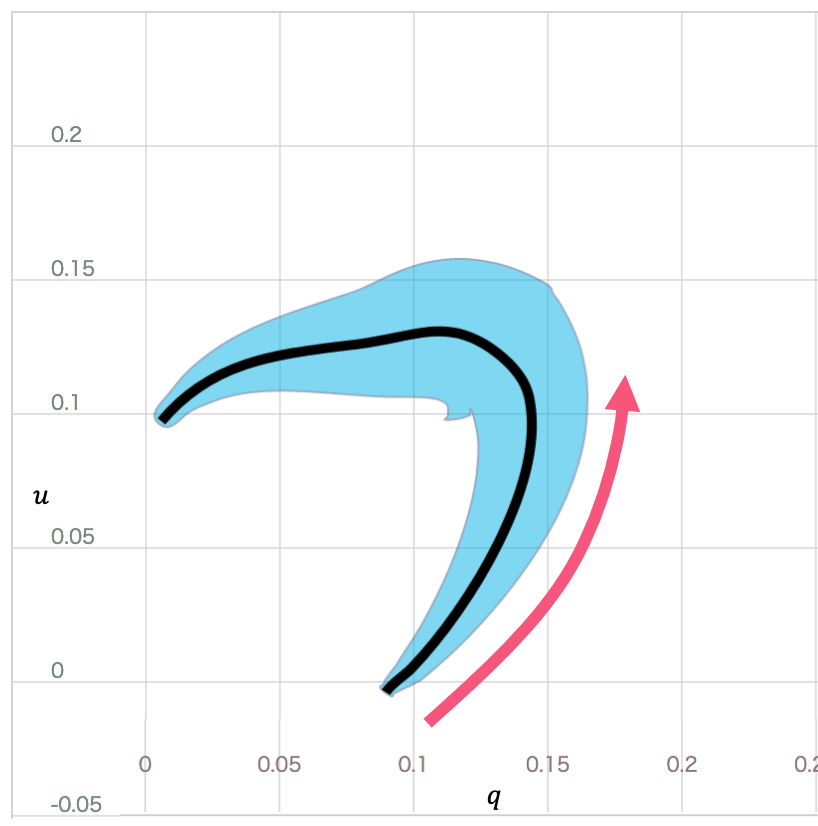
\includegraphics[width=.9\linewidth]{figures/QBScorrelate.png}\\
        \footnotesize{\sf(a)~A query for a correlated $I$ and $PD$ variation.}\\
    \end{minipage}
    \begin{minipage}{0.49\linewidth}
        \centering
        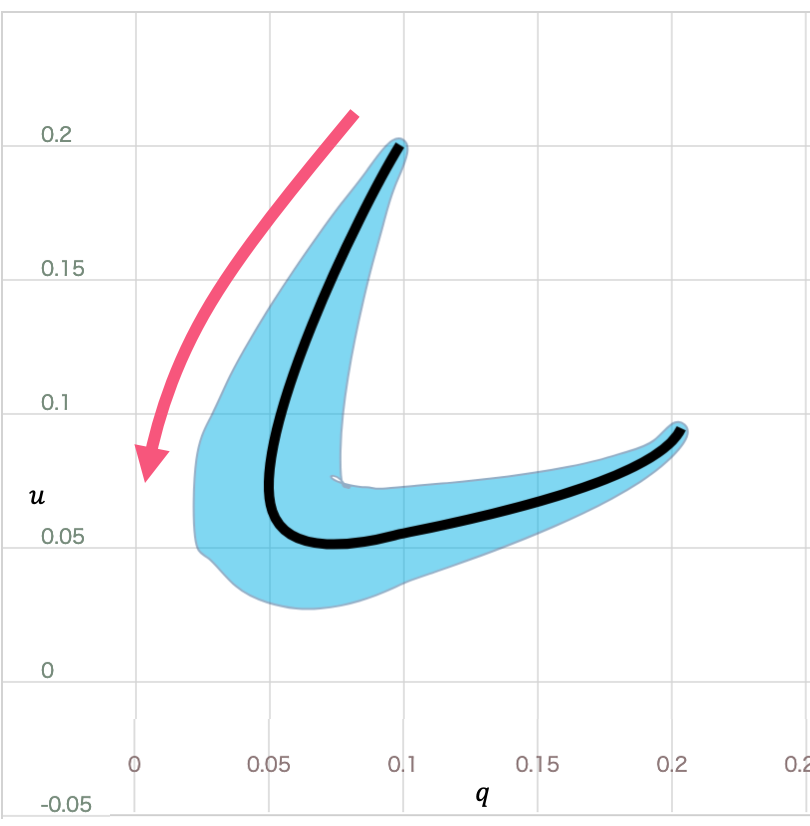
\includegraphics[width=.9\linewidth]{figures/QBSanticorrelate.png}\\
        \footnotesize{\sf(b)~A query for an anticorrelated $I$ and $PD$ variation.}\\
    \end{minipage}
    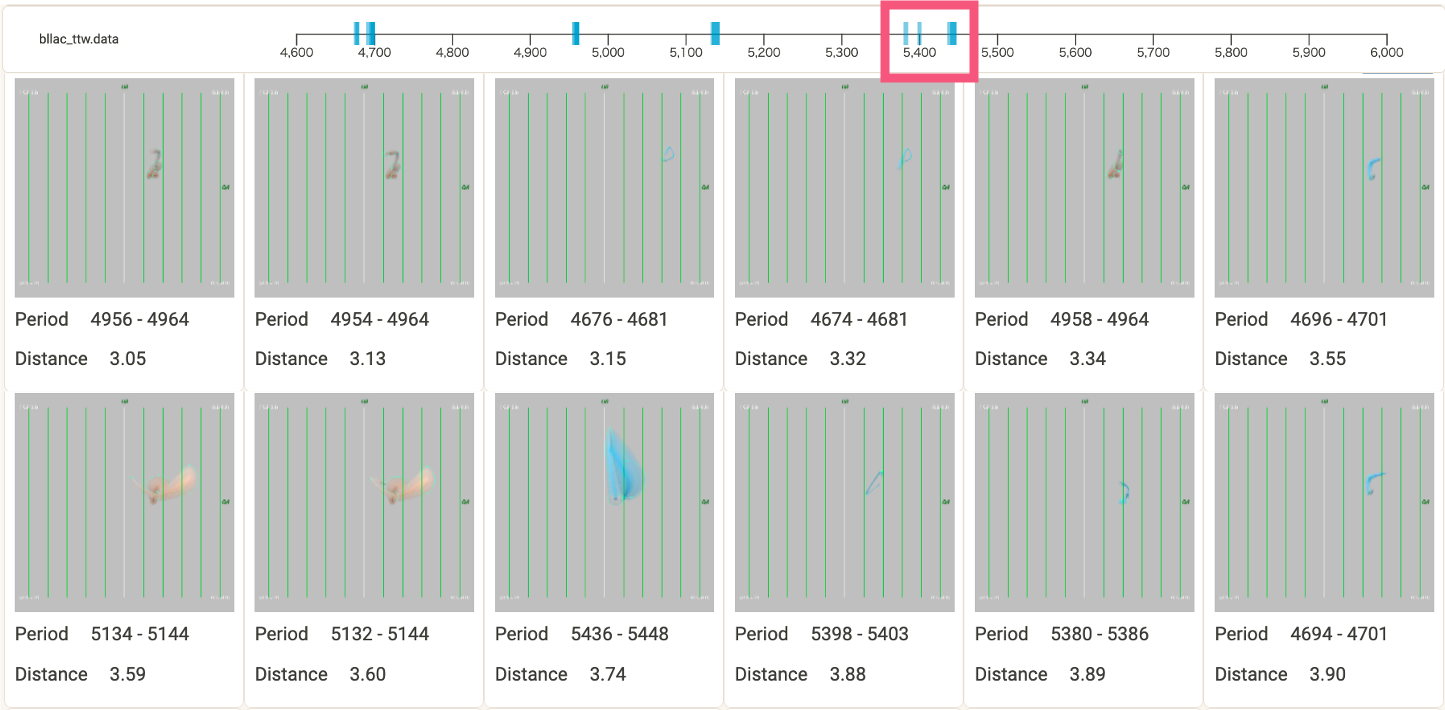
\includegraphics[width=.99\linewidth]{figures/correlateResultsLabel14.png}\\
    \footnotesize{\sf(c)~The top twelve time intervals that are similar to the query in (a).}\\
    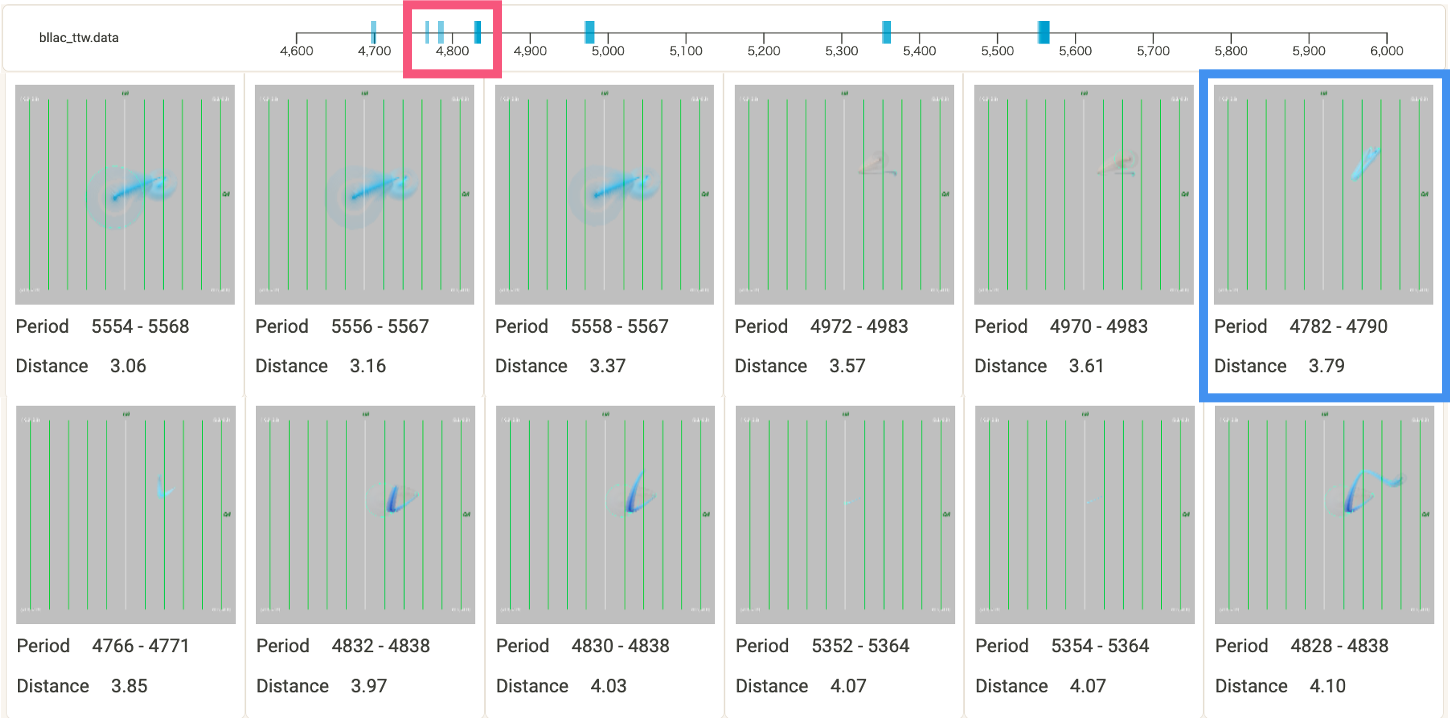
\includegraphics[width=.99\linewidth]{figures/anticorrelateResultsLabel14.png}\\
    \footnotesize{\sf(d)~The top twelve time intervals that are similar to the query in (b).}
    \caption{Analysis of the blazar \emph{BL Lac} to investigate correlation patterns between $I$ and $PD$. (a) and (b) are user-drawn sketches. (c) and (d) are the results of QBS with the queries shown in (a) and (b), respectively.}
    \label{fig:EvaluationQueryResults}
\end{figure}
%
Astronomer 1's goal in these case studies was to identify global statistical features of the period of interest and to build a hypothesis of correlations between the time variations of $I$ and $PD$.
To achieve this goal, he had to meticulously analyze correlations between $I$ and $PD$ in the entire time period and many short time intervals within that period.
However, it seemed difficult to manually examine each of the short time intervals.
Therefore, he decided to utilize QBS to investigate correlation patterns in a long-term observation dataset.

First, he formulated a hypothesis that an increase in $I$ tends to correlate with an increase in $PD$ in \emph{BL Lac}.
To validate this hypothesis and examine how frequently such behavior appears, he sketched the query shown in Fig.~\ref{fig:EvaluationQueryResults}~(a), 
where the $x$ and $y$ axes express $q$ and $u$, respectively, 
and the stroke width represents $I$.
Therefore, the input sketch indicates a pattern 
that $I$ gradually increases and then decreases in a way that is correlated to $PD$.
To extract time intervals with a similar shape but different position or different scale, he used the normalization and polar coordinates options. 
To avoid missing short events, he set the warping window size and the sliding window size to 0 and 2, respectively.

Fig.~\ref{fig:EvaluationQueryResults}~(c) shows the top twelve results of the query sketched in (a).
The timeline at the top of (c) illustrates 
that the extracted time intervals seem to be distributed over the entire dataset.
However, in the period from $[5{,}350, 5{,}450]$ (enclosed by a red rectangle in (c)), 
the input pattern seems to occur more frequently than in other periods.
Visiting all time intervals in this period individually and analyzing them in the TimeTubes view,
some of them include the correlation pattern in (a),
but others do not.
Thus, he concluded that the input correlation pattern does not frequently occur in that period.
The reason for this misclassification could be that our system, when using the normalization option, detects time intervals with a relatively small variation of $I$ as well.
However, he was still highly pleased with TimeTubesX, as it allowed him to quickly identify a relatively small number of time intervals that he could then examine in more detail.

\subsection{Case Study 2: Anticorrelation Patterns of $I$ and $PD$}\label{sec:anticorrelate}
Astronomer 1 also noticed that the variation in $I$ tends to anticorrelate with that in $PD$.
To detect time intervals with such anticorrelated $I$ and $PD$ patterns, he drew another query (Fig.~\ref{fig:EvaluationQueryResults}~(b))
where the plane represents the Stokes plane and the stroke width $I$.
The sketch describes a pattern in which $I$ gradually increases and then decreases, while $PD$ shows a negative correlation with $I$. 
He used the same parameters as in Section~\ref{sec:correlate}.

Fig.~\ref{fig:EvaluationQueryResults}~(d) shows the top twelve results of the query shown in (b).
Like in the previous case study, 
extracted time intervals seem to be distributed over the entire dataset.
However, in the period from $[4{,}750, 4{,}850]$ (enclosed by a red rectangle in (d)), 
the input pattern seems to occur more frequently.
Astronomer~1's group previously reported that, statistically, the variation in $I$ anticorrelates with that in $PD$ from the years 2008 to 2010 in \emph{BL Lac}~\cite{Gaur2014}.
However, even in that previous report, they did not analyze short time intervals in the period individually.
By analyzing the extracted time intervals in the period with TimeTubesX, he could verify not only that an increase in $I$ globally tends to co-occur with a decrease in $PD$, 
but also that local peaks of $I$ are correlated with decreases in $PD$.

These case studies with QBS underline the importance of local analysis of short time intervals within a larger time period in addition to a global analysis of the entire period.

\subsection{What-If Scenario Analysis}\label{sec:whatif}
This section explains how astronomers can identify what generally contributes to the $PD$ variation in blazars in a certain time period. 

Astronomers expect that $PD$ variation in a blazar is due to one of the two following hypotheses:
\begin{enumerate}[nosep, label=\textsl{Hypothesis \arabic*}:, ref=\textsl{Hypothesis \arabic*}, align=parleft, leftmargin=*]
    \item \textsl{$total\,flux$ increases (decreases) due to the increase (decrease) in $unpolarized\,flux$};  \label{scenario1}
    \item \textsl{There are two polarized components, and they are perpendicular to each other}. \label{scenario2}
\end{enumerate}
Note that $PD$ can be derived from the amount of $flux$: $PD = \frac{polarized\,flux}{total\,flux}$,
where $total flux = I = polarized\,flux + unpolarized\,flux$.
Astronomers can identify which of the above hypotheses contributes to the decrease in $PD$
by comparing time variations of data samples at the time intervals in the $q - u$ domain and in the $Q-U$ domain,
where $q = Q / I$ and $u = U / I$, as explained in Section~\ref{sec:BlazarData}.
In the case of \ref{scenario1}, the position of a data sample in the $q - u$ domain gradually moves toward the origin ($(q, u) = (0, 0)$),
whereas the position in the $Q-U$ domain does not move toward the origin ($(Q, U) = (0, 0)$)
because only the amount of $total flux$ increases.
On the other hand, in the case of \ref{scenario2}, 
$PD$ decreases due to a flare of another polarized component with $PA$ being perpendicular to the jet direction.
The position of a data sample moves toward the origin both in the $q - u$ domain and in the $Q - U$ domain 
because another polarized component influences the observed $Q$ and $U$ values, 
meaning that $q$ and $u$ (fractional values of $Q$ and $U$) are also influenced.
By comparing the datasets for $(q, u)$ and $(Q, U)$ with the side-by-side option in the visual data fusion~\cite{Fujishiro2018},
the plausibility of these hypotheses can be visually determined.
\begin{figure}[tb]
    \centering
    \includegraphics[width=.8\linewidth]{figures/stokesComparisonLabel.png}
    \caption{Comparison of a dataset consisting of $q$ and $u$ (left) and one consisting of $Q$ and $U$ (right) for the time interval $[4{,}782, 4{,}890]$.
    In both images, the position of the data sample goes toward the origin of the domain (lower left), which means that this polarization variation was caused by a decrease in the $PD$ of a different polarized component.}
    \label{fig:comparisonQIUIvsQU}
\end{figure}

The following discussion considers the anticorrelation patterns of $I$ and $PD$, as mentioned in Section~\ref{sec:anticorrelate}.
Astronomer 1 compared a dataset consisting of $q$ and $u$ with one consisting of $Q$ and $U$. The comparison results at the time interval with a blue rectangle displayed in Fig.~\ref{fig:EvaluationQueryResults}~(d) are shown in Fig.~\ref{fig:comparisonQIUIvsQU}.
As the red arrows in Fig.~\ref{fig:comparisonQIUIvsQU} indicate, 
he found that both data samples move toward the origin.
He found similar behavior at all short time intervals in the period $[4{,}750, 4{,}850]$.
Thus, he finally concluded that the negative correlation of $I$ and $PD$ in the period is not due to the increase in $unpolarized flux$ (\ref{scenario1}) but is instead due to the presence of two polarized components (\ref{scenario2}). 

Overall, TimeTubesX greatly facilitated this detailed visual exploration of blazar data. This allowed Astronomer 1 to examine many small time intervals with specific features, which would have been too laborious with previous methods.

\subsection{Qualitative Feedback from Domain Experts}\label{sec:feedback}
Astronomer 2 found that the rotation detection was useful. 
With TimeTubesX's rotation detection functionality, 
he was able to find three unknown rotation behaviors with a shifted rotation center in the blazar \emph{3C 454.3}~\cite{Huang2019}. 
Astronomers 1, 3, and 4 mentioned that the QBS method was especially useful and helpful for validating their high-level hypotheses, as demonstrated in Sections~\ref{sec:correlate} and \ref{sec:anticorrelate}. 
In particular, Astronomers 3 and 4 said that dynamic visual querying could be a powerful tool to examine jet physical processes and behaviors of plasma and magnetic fields under extreme conditions because the method can efficiently address arbitrary variation patterns of polarization, intensity, and color over time. Astronomers 1 and 3 noticed TimeTubesX’s potential for data mining. In particular, Astronomer 3 saw massive potential for mining existing and upcoming large polarization surveys, while Astronomer 1 found that using TimeTubesX will enable astronomers to identify interesting features in short time intervals to an extent that cannot be achieved with conventional methods due to too many short time intervals in a long-term dataset. Furthermore, fact-guided querying was impressive to him because it allows astronomers to refine their sketches based on actual extracted patterns.

\section{Conclusion and future work\label{sec:conclusion}}
We have presented a web-based visual analytics environment for the detailed analysis of blazar datasets, termed TimeTubesX. 
TimeTubesX is expected to facilitate astronomers’ analysis of photometric and polarimetric behaviors of blazars 
by enabling automatic feature extraction and dynamic visual querying.
It allows astronomers not only to easily locate observable blazar behaviors but also to efficiently find recurring time variation patterns.
TimeTubesX has the potential to allow astronomers to find short time variation patterns that have not yet been discovered.

In the future, 
to avoid undesirable effects of outliers,
we should take observation errors into account during the feature extraction processes. 
We should also consider provenance management to holistically keep track of users’ analysis processes, as realized in aflak~\cite{Boussejra2019}.
Furthermore, we would like to incorporate a deep learning approach to classify time series data in a non-biased manner because the current query specification process in QBE and QBS significantly depends on users' expertise.
To provide a more effective overview of the results, it would also be helpful to cluster the results of a query. 
Applying TimeTubesX to multi-dimensional, time-dependent datasets in other domains will likely form yet another part of our future research.


% \IEEEraisesectionheading{\section{Introduction}\label{sec:introduction}}
% % Computer Society journal (but not conference!) papers do something unusual
% % with the very first section heading (almost always called "Introduction").
% % They place it ABOVE the main text! IEEEtran.cls does not automatically do
% % this for you, but you can achieve this effect with the provided
% % \IEEEraisesectionheading{} command. Note the need to keep any \label that
% % is to refer to the section immediately after \section in the above as
% % \IEEEraisesectionheading puts \section within a raised box.




% % The very first letter is a 2 line initial drop letter followed
% % by the rest of the first word in caps (small caps for compsoc).
% % 
% % form to use if the first word consists of a single letter:
% % \IEEEPARstart{A}{demo} file is ....
% % 
% % form to use if you need the single drop letter followed by
% % normal text (unknown if ever used by the IEEE):
% % \IEEEPARstart{A}{}demo file is ....
% % 
% % Some journals put the first two words in caps:
% % \IEEEPARstart{T}{his demo} file is ....
% % 
% % Here we have the typical use of a "T" for an initial drop letter
% % and "HIS" in caps to complete the first word.
% \IEEEPARstart{T}{his} demo file is intended to serve as a ``starter file''
% for IEEE Computer Society journal papers produced under \LaTeX\ using
% IEEEtran.cls version 1.8b and later.
% % You must have at least 2 lines in the paragraph with the drop letter
% % (should never be an issue)
% I wish you the best of success.

% \hfill mds
 
% \hfill August 26, 2015

% \subsection{Subsection Heading Here}
% Subsection text here.

% % needed in second column of first page if using \IEEEpubid
% %\IEEEpubidadjcol

% \subsubsection{Subsubsection Heading Here}
% Subsubsection text here.


% % An example of a floating figure using the graphicx package.
% % Note that \label must occur AFTER (or within) \caption.
% % For figures, \caption should occur after the \includegraphics.
% % Note that IEEEtran v1.7 and later has special internal code that
% % is designed to preserve the operation of \label within \caption
% % even when the captionsoff option is in effect. However, because
% % of issues like this, it may be the safest practice to put all your
% % \label just after \caption rather than within \caption{}.
% %
% % Reminder: the "draftcls" or "draftclsnofoot", not "draft", class
% % option should be used if it is desired that the figures are to be
% % displayed while in draft mode.
% %
% %\begin{figure}[!t]
% %\centering
% %\includegraphics[width=2.5in]{myfigure}
% % where an .eps filename suffix will be assumed under latex, 
% % and a .pdf suffix will be assumed for pdflatex; or what has been declared
% % via \DeclareGraphicsExtensions.
% %\caption{Simulation results for the network.}
% %\label{fig_sim}
% %\end{figure}

% % Note that the IEEE typically puts floats only at the top, even when this
% % results in a large percentage of a column being occupied by floats.
% % However, the Computer Society has been known to put floats at the bottom.


% % An example of a double column floating figure using two subfigures.
% % (The subfig.sty package must be loaded for this to work.)
% % The subfigure \label commands are set within each subfloat command,
% % and the \label for the overall figure must come after \caption.
% % \hfil is used as a separator to get equal spacing.
% % Watch out that the combined width of all the subfigures on a 
% % line do not exceed the text width or a line break will occur.
% %
% %\begin{figure*}[!t]
% %\centering
% %\subfloat[Case I]{\includegraphics[width=2.5in]{box}%
% %\label{fig_first_case}}
% %\hfil
% %\subfloat[Case II]{\includegraphics[width=2.5in]{box}%
% %\label{fig_second_case}}
% %\caption{Simulation results for the network.}
% %\label{fig_sim}
% %\end{figure*}
% %
% % Note that often IEEE papers with subfigures do not employ subfigure
% % captions (using the optional argument to \subfloat[]), but instead will
% % reference/describe all of them (a), (b), etc., within the main caption.
% % Be aware that for subfig.sty to generate the (a), (b), etc., subfigure
% % labels, the optional argument to \subfloat must be present. If a
% % subcaption is not desired, just leave its contents blank,
% % e.g., \subfloat[].


% % An example of a floating table. Note that, for IEEE style tables, the
% % \caption command should come BEFORE the table and, given that table
% % captions serve much like titles, are usually capitalized except for words
% % such as a, an, and, as, at, but, by, for, in, nor, of, on, or, the, to
% % and up, which are usually not capitalized unless they are the first or
% % last word of the caption. Table text will default to \footnotesize as
% % the IEEE normally uses this smaller font for tables.
% % The \label must come after \caption as always.
% %
% %\begin{table}[!t]
% %% increase table row spacing, adjust to taste
% %\renewcommand{\arraystretch}{1.3}
% % if using array.sty, it might be a good idea to tweak the value of
% % \extrarowheight as needed to properly center the text within the cells
% %\caption{An Example of a Table}
% %\label{table_example}
% %\centering
% %% Some packages, such as MDW tools, offer better commands for making tables
% %% than the plain LaTeX2e tabular which is used here.
% %\begin{tabular}{|c||c|}
% %\hline
% %One & Two\\
% %\hline
% %Three & Four\\
% %\hline
% %\end{tabular}
% %\end{table}


% % Note that the IEEE does not put floats in the very first column
% % - or typically anywhere on the first page for that matter. Also,
% % in-text middle ("here") positioning is typically not used, but it
% % is allowed and encouraged for Computer Society conferences (but
% % not Computer Society journals). Most IEEE journals/conferences use
% % top floats exclusively. 
% % Note that, LaTeX2e, unlike IEEE journals/conferences, places
% % footnotes above bottom floats. This can be corrected via the
% % \fnbelowfloat command of the stfloats package.




% \section{Conclusion}
% The conclusion goes here.





% % if have a single appendix:
% %\appendix[Proof of the Zonklar Equations]
% % or
% %\appendix  % for no appendix heading
% % do not use \section anymore after \appendix, only \section*
% % is possibly needed

% % use appendices with more than one appendix
% % then use \section to start each appendix
% % you must declare a \section before using any
% % \subsection or using \label (\appendices by itself
% % starts a section numbered zero.)
% %


% \appendices
% \section{Proof of the First Zonklar Equation}
% Appendix one text goes here.

% % you can choose not to have a title for an appendix
% % if you want by leaving the argument blank
% \section{}
% Appendix two text goes here.


% % use section* for acknowledgment
\ifCLASSOPTIONcompsoc
  % The Computer Society usually uses the plural form
  \section*{Acknowledgments}
\else
  % regular IEEE prefers the singular form
  \section*{Acknowledgment}
\fi
The authors have benefited from useful discussions with Mahito Sasada at Hiroshima University, Yannis Liodakis at Stanford University, and Alan Marscher, Svetlana Jorstad, Manasvita Joshi, and Zachary Weaver at Boston University.
We would like to thank Carolina Nobre at Harvard University for inserting the narration into the accompanying video.
The present work has been financially supported in part by a MEXT KAKENHI Grant-in-Aid for Scientific Research(A) No. 17H00737 and King Abdullah
University of Science and Technology (KAUST) and the KAUST Office of Sponsored
Research (OSR)'s award, OSR-2015-CCF-2533-0.
Sawada, the first author, would also like to thank the Yoshida Scholarship Foundation.


% Can use something like this to put references on a page
% by themselves when using endfloat and the captionsoff option.
\ifCLASSOPTIONcaptionsoff
  \newpage
\fi



% trigger a \newpage just before the given reference
% number - used to balance the columns on the last page
% adjust value as needed - may need to be readjusted if
% the document is modified later
%\IEEEtriggeratref{8}
% The "triggered" command can be changed if desired:
%\IEEEtriggercmd{\enlargethispage{-5in}}

% references section

% can use a bibliography generated by BibTeX as a .bbl file
% BibTeX documentation can be easily obtained at:
% http://mirror.ctan.org/biblio/bibtex/contrib/doc/
% The IEEEtran BibTeX style support page is at:
% http://www.michaelshell.org/tex/ieeetran/bibtex/
% \bibliographystyle{IEEEtran}
% argument is your BibTeX string definitions and bibliography database(s)
%\bibliography{IEEEabrv,../bib/paper}
%
% <OR> manually copy in the resultant .bbl file
% set second argument of \begin to the number of references
% (used to reserve space for the reference number labels box)

% \bibliography{IEEEabrv,references}


\bibliographystyle{IEEEtran}
\bibliography{IEEEabrv,references}
% \begin{thebibliography}{1}

% \bibitem{IEEEhowto:kopka}
% H.~Kopka and P.~W. Daly, \emph{A Guide to \LaTeX}, 3rd~ed.\hskip 1em plus
%   0.5em minus 0.4em\relax Harlow, England: Addison-Wesley, 1999.

% \end{thebibliography}

% biography section
% 
% If you have an EPS/PDF photo (graphicx package needed) extra braces are
% needed around the contents of the optional argument to biography to prevent
% the LaTeX parser from getting confused when it sees the complicated
% \includegraphics command within an optional argument. (You could create
% your own custom macro containing the \includegraphics command to make things
% simpler here.)
%\begin{IEEEbiography}[{\includegraphics[width=1in,height=1.25in,clip,keepaspectratio]{mshell}}]{Michael Shell}
% or if you just want to reserve a space for a photo:

\begin{IEEEbiography}[{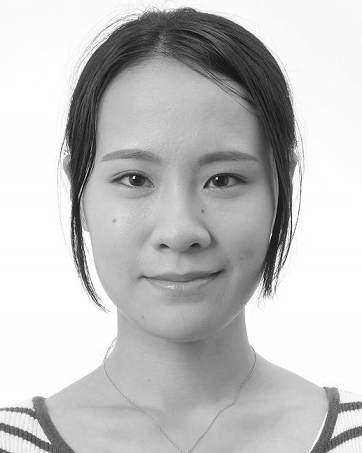
\includegraphics[width=1in,height=1.25in,clip,keepaspectratio]{bio/naoko_BW.jpg}}]{Naoko Sawada}
received BE and ME degrees in information and computer science from Keio University in 2017 and 2018, respectively. 
She is currently working toward a PhD degree 
at the School of Science for Open and Environmental Systems, Keio University.
% in Graduate School of Science and Technology, Keio University.
She stayed at Harvard University as a visiting scholar in the Visual Computing Group from 2018 to 2020.
Her main research interests are time-varying multi-dimensional data visualization and analytics.
\end{IEEEbiography}

% if you will not have a photo at all:
\begin{IEEEbiography}[{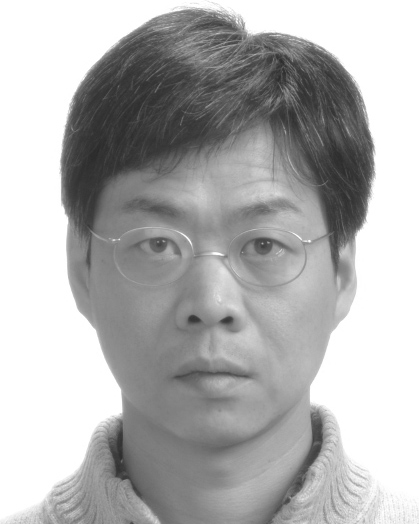
\includegraphics[width=1in,height=1.25in,clip,keepaspectratio]{bio/Uemura_BW.jpg}}]{Makoto Uemura}
received a PhD degree from 
Kyoto University, Japan, in 2004 for research on
astrophysics. He is an associate professor at 
Hiroshima Astrophysical Science Center, 
Hiroshima University. His research interests include
physics of astronomical variable stars, data science, 
and visual analytics for astronomy. He is especially 
interested in the analysis of high-dimensional data 
concerning black hole systems. 
\end{IEEEbiography}

% insert where needed to balance the two columns on the last page with
% biographies
%\newpage

\begin{IEEEbiography}[{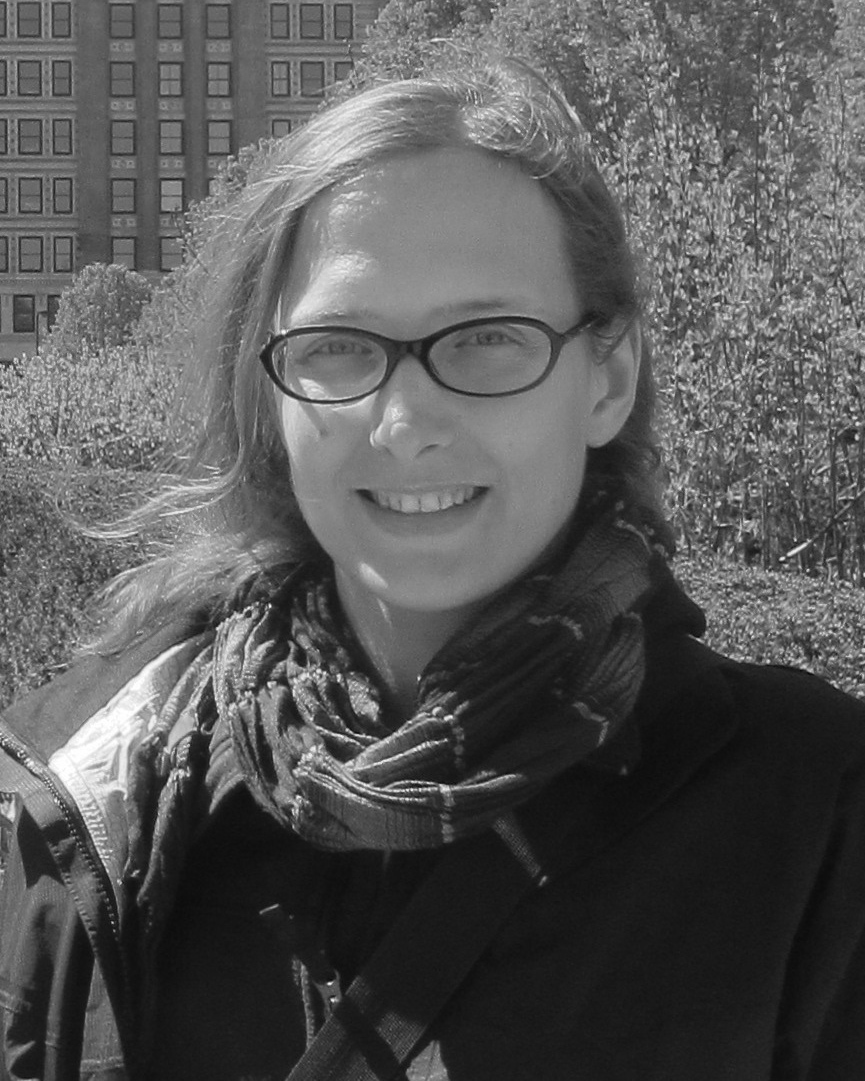
\includegraphics[width=1in,height=1.25in,clip,keepaspectratio]{bio/johanna_BW.jpg}}]{Johanna Beyer}
is a research associate in the School of Engineering and Applied Sciences at Harvard University. Before joining Harvard, she was a postdoctoral fellow at the Geometric Modeling and Scientific Visualization Center at King Abdullah University of Science and Technology. Her research interests include large-data visualization, GPU-based volume rendering, and the combination of abstract information visualization with scientific visualization for novel domain-specific applications. She received a PhD in computer science from the Vienna University of Technology in 2010.
\end{IEEEbiography}

\begin{IEEEbiography}[{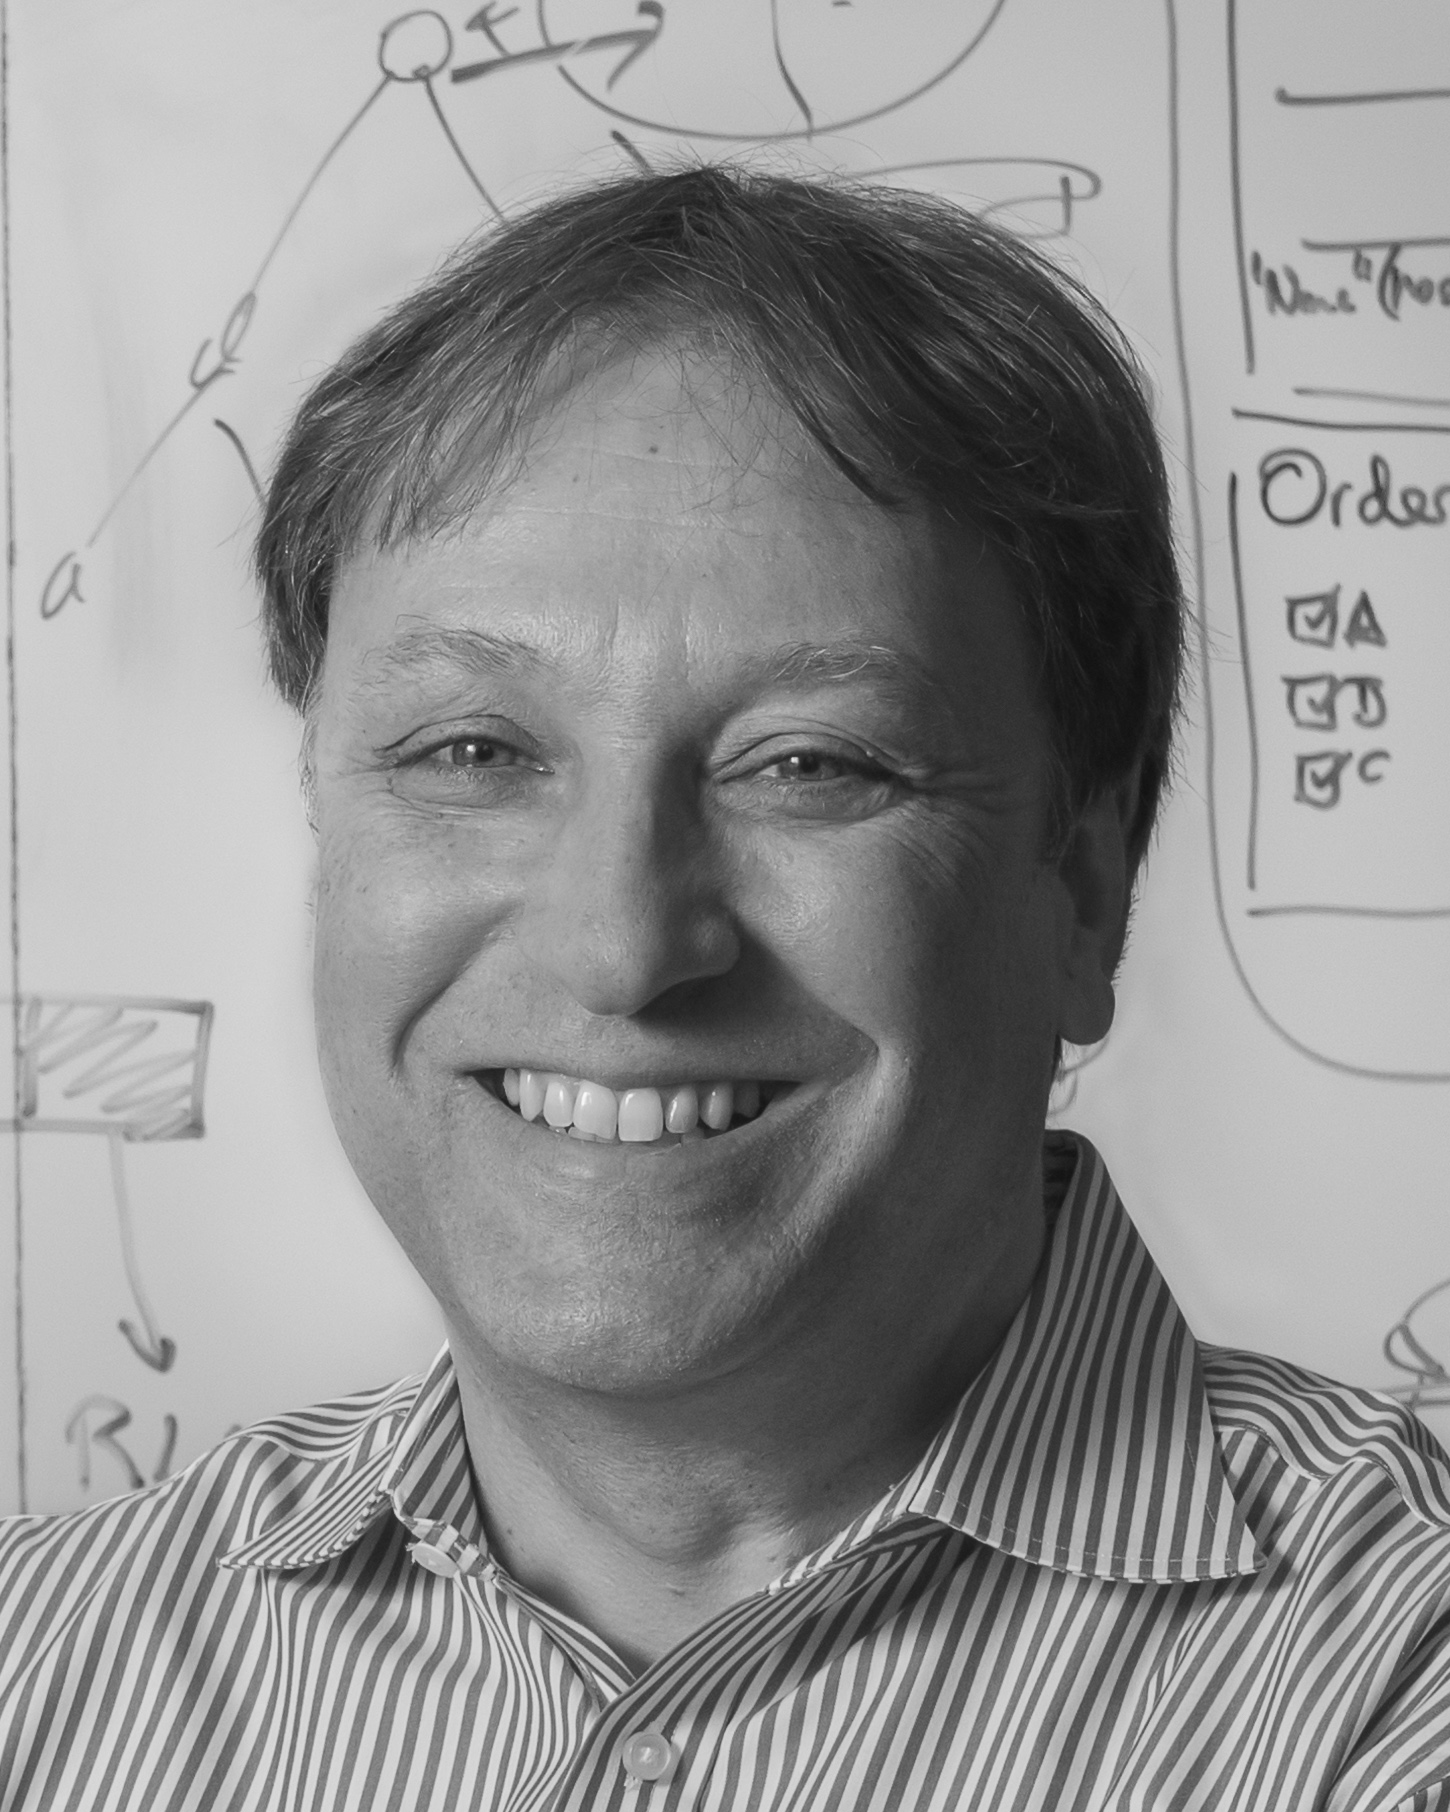
\includegraphics[width=1in,height=1.25in,clip,keepaspectratio]{bio/HP_BW.jpg}}]{Hanspeter Pfister}
is the An Wang Professor of Computer Science at the Harvard John A. Paulson School of Engineering and Applied Sciences and an affiliate faculty member of the Center for Brain Science. His research in visual computing lies at the intersection of visualization, computer graphics, and computer vision and spans a wide range of topics, including biomedical image analysis and visualization, image and video analysis, interpretable machine learning, and visual analytics in data science. Pfister has a PhD in computer science from the State University of New York at Stony Brook and an MS in electrical engineering from ETH Zurich, Switzerland. From 2013 to 2017, he was the director of the Institute for Applied Computational Science. 
Before joining Harvard, he worked for over a decade at Mitsubishi Electric Research Laboratories, where he was an associate director and senior research scientist. 
He was the chief architect of VolumePro, Mitsubishi Electric’s award-winning real-time volume rendering graphics card, for which he received the Mitsubishi Electric President’s Award in 2000. Pfister was elected as an ACM Fellow in 2019. 
% He is the recipient of the 2010 IEEE Visualization Technical Achievement Award, the 2009 IEEE Meritorious Service Award, and the 2009 Petra T. Shattuck Excellence in Teaching Award. Pfister is a member of the ACM SIGGRAPH Academy, the IEEE Visualization Academy, and a director of the IEEE Visualization and Graphics Technical Committee.
\end{IEEEbiography}

\begin{IEEEbiography}[{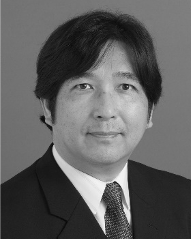
\includegraphics[width=1in,height=1.25in,clip,keepaspectratio]{bio/issei_BW.png}}]{Issei Fujishiro}
is a professor at the Department of Information and Computer Science, Faculty of Science and Technology, Keio University. He is also an adjunct professor at the School of Computer Science and Technology, Hangzhou Dianzi University. 
Before joining Keio University in 2009, he held faculty positions at the University of Tokyo, University of Tsukuba, Ochanomizu University, and Tohoku University. He stayed as a visiting professor at the State University of New York at Stony Brook from 1994 to 1995. 
He received a Doctor of Science degree in information sciences from the University of Tokyo in 1988. His research interests include modeling paradigms and shape representations, applied visualization design and lifecycle management, and smart ambient media with multi-modal displays. He has served as an associate editor for \textit{IEEE TVCG} and the \textit{Elsevier Journal of Visual Informatics}. 
% He was a paper co-chair (SciVis) for VIS 2019/2018.
He has chaired 35 international conferences on visualization and computer graphics,
acting as a paper co-chair (SciVis) for IEEE VIS 2019/2018 and as a
workshop co-chair for PacificVAST 2018 and TopoInVis 2017.
Fujishiro is a member of the Science Council of Japan.
% received his Doctor of Science in information sciences from the University of Tokyo in 1988. He joined Keio University in 2009, where he is currently a Professor at Department of Information and Computer Science, Faculty of Science and Technology. He is also an Adjunct Professor at School of Computer Science and Engineering, Hangzhou Dianzi University. His research interests include modeling paradigms and shape representations, applied visualization design and lifecycle management, and smart ambient media with multi-modal displays. He has been serving as an associate editor for IEEE Transactions on Visualization and Computer Graphics and Elsevier Journal of Visual Informatics, and on the steering committee for IEEE SciVis and IEEE PacificVis. He chaired more than 35 international conferences on visualization and computer graphics, including a paper co-chair for SciVis 2019/2018, a workshop chair for PacificVAST 2018 and TopoInVis 2017. Fujishiro is a member of Science Council of Japan.
\end{IEEEbiography}
% You can push biographies down or up by placing
% a \vfill before or after them. The appropriate
% use of \vfill depends on what kind of text is
% on the last page and whether or not the columns
% are being equalized.

%\vfill

% Can be used to pull up biographies so that the bottom of the last one
% is flush with the other column.
%\enlargethispage{-5in}



% that's all folks
\end{document}


